% TODO: Można zmienić na angielski wybierając drugą linię
\documentclass[11pt]{aghdpl}

% TODO:
% Lista wszystkich języków stanowiących języki pozycji bibliograficznych użytych w pracy.
% (Zgodnie z zasadami tworzenia bibliografii każda pozycja powinna zostać utworzona zgodnie z zasadami języka, w którym dana publikacja została napisana.)
\usepackage[english,polish]{babel}

% Użyj polskiego łamania wyrazów (zamiast domyślnego angielskiego).
% TODO: Można zmienić na angielski
\usepackage{polski}

\usepackage[utf8]{inputenc}

% dodatkowe pakiety

\usepackage{mathtools}
\usepackage{amsfonts}
\usepackage{amsmath}
\usepackage{amsthm}
\usepackage{float} 
\usepackage{realboxes}
\usepackage{xpatch}

%Landscape
\usepackage{lscape}

%Do dodawnaie stron pdf jako część dokumentu (nie lstlisting)
\usepackage{pdfpages}

% Paczka wyłącza pokazywanie numeru strony oraz nagłówków na pustych stronach
% TODO: Można wyłączyć
\usepackage{emptypage}

% Dodatkowe kolory:
\usepackage{colortbl}
\definecolor{redi}{RGB}{255,38,0}
\definecolor{redii}{RGB}{200,50,30}
\definecolor{yellowi}{RGB}{255,251,0}
\definecolor{bluei}{RGB}{0,150,255}
\definecolor{blueii}{RGB}{135,247,210}
\definecolor{blueiii}{RGB}{91,205,250}
\definecolor{blueiv}{RGB}{115,244,253}
\definecolor{bluev}{RGB}{1,58,215}
\definecolor{orangei}{RGB}{240,143,50}
\definecolor{yellowii}{RGB}{222,247,100}
\definecolor{greeni}{RGB}{166,247,166}
\definecolor{gray}{RGB}{200, 200, 200}
\definecolor{lgray}{RGB}{240, 240, 240}

\usepackage{siunitx}

% Dzięki temu będzie się dało kopiować tekst który ma polskie literki
% see: https://tex.stackexchange.com/questions/57915/cannot-copy-letters-with-diacritics-from-pdflatex-pdf
\usepackage{lmodern}
\usepackage{listings}


% Polskie literki w listingach:
\lstset{
    literate=
    {ą}{{\k{a}}}1 {Ą}{{\k{A}}}1 
    {ł}{{\l{}}}1 {Ł}{{\L{}}}1 
    {ń}{{\'n}}1 {Ń}{{\'N}}1 
    {ę}{{\k{e}}}1 {Ę}{{\k{E}}}1 
    {ś}{{\'s}}1 {Ś}{{\'S}}1 
    {ż}{{\.z}}1 {Ż}{{\.Z}}1 
    {ó}{{\'o}}1 {Ó}{{\'O}}1 
    {ź}{{\'z}}1 {Ź}{{\'Z}}1 
    {ć}{{\'c}}1 {Ć}{{\'C}}1
}


% Definicja listingu dla Dockerfile
% https://gordonlesti.com/custom-code-highlighting-in-latex/
\lstdefinelanguage{Dockerfile}
{
  morekeywords={FROM, RUN, CMD, LABEL, MAINTAINER, EXPOSE, ENV, ADD, COPY,
    ENTRYPOINT, VOLUME, USER, WORKDIR, ARG, ONBUILD, STOPSIGNAL, HEALTHCHECK,
    SHELL},
  morecomment=[l]{\#},
  morestring=[b]"
}

% Definicja listingu dla CMAKE
\lstdefinelanguage{cmake}
{
  morekeywords={set, cmake_minimum_required, project, add_executable, target_include_directories, include, target_link_libraries, file, add_library, set_target_properties, if, endif, list, foreach, endforeach, add_subdirectory, get_directory_property, get_filename_component, function, endfunction, execute_process, ExternalProject_Add, target_link_directories},
  morecomment=[l]{\#},
  morestring=[b]"
}

\lstdefinelanguage{Cmd}
{
    moredelim=[s][\color{red}\bfseries]{user@host}{\$},
    morekeywords={}
}

\definecolor{darkgreenforcomments}{rgb}{0.0,0.26,0.15}

\lstdefinelanguage{yaml}
{
  keywords={true,false,null,y,n},
  sensitive=false,
  comment=[l]{\#},
  morecomment=[s]{/*}{*/},
  commentstyle=\color{darkgreenforcomments}\ttfamily,
  stringstyle={\color{blue}\mdseries},
  moredelim=[l][\color{orange}]{\&},
  moredelim=[l][\color{magenta}]{*},
  moredelim=**[il][\color{red}{:}\color{blue}]{:},
  morestring=[b]',
  morestring=[b]"
}

\definecolor{lgray}{gray}{0.96}
\definecolor{lbcolor}{rgb}{0.9,0.9,0.9}
\lstset{
    framesep=2pt,
    basicstyle=\ttfamily,
    breaklines=true,
    breakatwhitespace=true,
    basicstyle=\footnotesize,
    aboveskip={0.75\baselineskip},
    columns=fixed,
    showstringspaces=false,
    breaklines=true,
    prebreak = \raisebox{0ex}[0ex][0ex]{\ensuremath{\hookleftarrow}},
    frame=single,
    rulecolor=\color{lgray},
    showtabs=false,
    showspaces=false,
    showstringspaces=false,
    backgroundcolor=\color{lgray},
    identifierstyle=\ttfamily,
    keywordstyle=\color[rgb]{0,0,1},
    commentstyle=\color[rgb]{0.0,0.26,0.15},
    stringstyle=\color[rgb]{0.627,0.126,0.941}
}

% Padding w podpisach do listingow i obrazkow
% ustawiony na 0
\captionsetup[lstlisting]{ margin=0pt}
\captionsetup[figure]{ margin=0pt}
\captionsetup[table]{ margin=0pt}



\makeatletter
\xpretocmd\lstinline{\Colorbox{lgray}\bgroup\appto\lst@DeInit{\egroup}}{}{}
\makeatother

\usepackage[hidelinks]{hyperref}

% --- < bibliografia > ---
%
% TODO: Dla TeXstudio warto przeczytać poniższe!
% UWAGA: Żeby bibliografia działała gdy używamy TeXstudio, to należy zmodyfikować quick build w opcjach, tak aby wykonywane były polecenia:
% 	PdfLaTeX
% 	BibTeX
% 	PdfLaTeX
% 	PdfLaTeX
%
% Więcej informacji na:
% 	https://tex.stackexchange.com/a/216325
%

\usepackage[
	backend=bibtex,
	style=numeric,
	sorting=none,
	% Zastosuj styl wpisu bibliograficznego właściwy językowi publikacji.
	language=autobib,
	autolang=other,
	% Zapisuj datę dostępu do strony WWW w formacie RRRR-MM-DD.
	urldate=iso8601,
	% Nie dodawaj numerów stron, na których występuje cytowanie.
	backref=false,
	% Podawaj ISBN.
	isbn=true,
	% Nie podawaj URL-i, o ile nie jest to konieczne.
	url=false,
	% Ustawienia związane z polskimi normami dla bibliografii.
	maxnames=50,
]{biblatex}

\usepackage{csquotes}
% Ponieważ `csquotes` nie posiada polskiego stylu, można skorzystać z mocno zbliżonego stylu chorwackiego.
\DeclareQuoteAlias{croatian}{polish}

% Bibliografia musi być uzupełniona w tym pliku:
\addbibresource{bibliografia.bib}

% Nie wyświetlaj wybranych pól.
%\AtEveryBibitem{\clearfield{note}}


% ------------------------
% --- < listingi > ---

% Użyj czcionki kroju Courier.
\usepackage{courier}

\lstloadlanguages{TeX}

% Polskie literki:
\lstset{
	literate={ą}{{\k{a}}}1
           {ć}{{\'c}}1
           {ę}{{\k{e}}}1
           {ó}{{\'o}}1
           {ń}{{\'n}}1
           {ł}{{\l{}}}1
           {ś}{{\'s}}1
           {ź}{{\'z}}1
           {ż}{{\.z}}1
           {Ą}{{\k{A}}}1
           {Ć}{{\'C}}1
           {Ę}{{\k{E}}}1
           {Ó}{{\'O}}1
           {Ń}{{\'N}}1
           {Ł}{{\L{}}}1
           {Ś}{{\'S}}1
           {Ź}{{\'Z}}1
           {Ż}{{\.Z}}1,
	basicstyle=\footnotesize\ttfamily,
}

% ------------------------
% Określamy nazwy 'table' oraz 'figure':
\AtBeginDocument{
	\renewcommand{\tablename}{Tabela}
	\renewcommand{\figurename}{Rys.}
}

% ------------------------
% --- < tabele > ---

% TODO: Dodatkowe paczki do tabel, można usunąć
\usepackage{tabularx}
\usepackage{multirow}
\usepackage{booktabs}
\usepackage{makecell}
\usepackage{float}


\usepackage[inline]{enumitem}
\setlist{nosep}

\usepackage{glossaries}

\newglossaryentry{git}{
  name=Git,
  description={}
}

\newglossaryentry{qt}{
  name=QT,
  description={}
}

\newglossaryentry{ggss}{
  name=GGSS,
  description={}
}

\newacronym{trt}{TRT}{Transition Radiation Tracker}

\newacronym{bash}{Bash}{Bourne Again Shell}

\newacronym{qwt}{QWT}{Qt Widgets}

\newacronym{cmake}{CMake}{Cross Platform Make}

\newacronym{svn}{SVN}{Subversion}

\newacronym{rpm}{RPM}{Red Hat Package Manager}

\newacronym{dim}{DIM}{Distributed Information Management System}

% defines the X column to use m (\parbox[c]) instead of p (`parbox[t]`)
\newcolumntype{C}[1]{>{\hsize=#1\hsize\centering\arraybackslash}X}


%---------------------------------------------------------------------------

% TODO: Poniższe mogą się wyświetlać lub nie w zależności od wariantów wyżej
% Np. języka lub innej konfiguracji
% Prawdopodobnie niektóre z poniższych nie są nigdy używane.
% Jeśli o tym wiesz, to warto rozwinąć ten szablon i udostępnić go dalej ;)

\author{Jarosław Cierpich \and Arkadiusz Kasprzak}
\shortauthor{}

\titlePL{Rozbudowa i uaktualnienie oprogramowania systemu GGSS detektora ATLAS TRT}
\titleEN{Update and upgrade of the GGSS system software for ATLAS TRT detector}

% Skrócone wersje tytułów po polsku/angielsku
% wyświetlane np. gdy normalne są bardzo długie
\shorttitlePL{Rozbudowa i uaktualnienie oprogramowania systemu GGSS detektora ATLAS TRT}

% Rodzaj pracy
\thesistype{Praca inżynierska}

% Promotor/opiekun pracy
\supervisor{dr hab. inż. Bartosz Mindur}

% Kierunek studiów
\degreeprogramme{Informatyka Stosowana}

% TODO: DATE
\date{2019/2020}

% Wydział
\faculty{Wydział Fizyki i Informatyki Stosowanej}


\setlength{\cftsecnumwidth}{10mm}

%---------------------------------------------------------------------------
\setcounter{secnumdepth}{4}

\begin{document}

% =====  STRONA TYTULOWA PRACY INŻYNIERSKIEJ ====
% ostatnia modyfikacja: 2011/03/09, K. Malarz

\thispagestyle{empty}

%% ------------------------ NAGLOWEK STRONY ---------------------------------

\includegraphics[height=37.5mm]{res/agh_nzw_a_pl_1w_wbr_cmyk.pdf}\\
\rule{30mm}{0pt}
{\Large\textsf{Wydział Fizyki i Informatyki Stosowanej}}\\
\rule{\textwidth}{3pt}\\
\rule[2.75ex]
{\textwidth}{1pt}%\\
\vspace{1em}\rule{30mm}{0pt}
\begin{center}
    {\bf\LARGE\textsf{Praca inżynierska}}\\
    \vspace{13ex}
    % --------------------------- IMIE I NAZWISKO -------------------------------
    {\bf\Large\textsf{Jarosław Cierpich \\ Arkadiusz Kasprzak}}\\
    \vspace{3ex}
    {\sf \small kierunek studiów:} {\bf\small\textsf{informatyka stosowana}}\\
    \vspace{15ex}
    %% ------------------------ TYTUL PRACY --------------------------------------
    {\bf\huge\textsf{Rozbudowa i uaktualnienie oprogramowania systemu GGSS detektora ATLAS TRT}}\\
    \vspace{14ex}
    %% ------------------------ OPIEKUN PRACY ------------------------------------
    {\sf \Large Opiekun:} {\bf\Large\textsf{dr hab. inż. Bartosz Mindur}}\\
    \vspace{22ex}
    \textsf{\bf\large\textsf{Kraków, styczeń 2020}}
\end{center}
%% =====  STRONA TYTUŁOWA PRACY INŻYNIERSKIEJ  ====

\newpage

%% =====  TYŁ STRONY TYTUŁOWEJ PRACY INŻYNIERSKIEJ  ====
\begin{center}
	{\bf\large\textsf{Oświadczenie studenta}}
\end{center}


{\sf Uprzedzony(-a) o odpowiedzialności karnej na podstawie art. 115 ust. 1 i 2 ustawy z dnia 4 lutego 1994 r. o prawie autorskim i prawach pokrewnych (t.j. Dz. U. z 2018 r. poz. 1191 z późn. zm.): ,,Kto przywłaszcza sobie autorstwo albo wprowadza w błąd co do autorstwa całości lub części cudzego utworu albo artystycznego wykonania, podlega grzywnie, karze ograniczenia wolności albo pozbawienia wolności do lat 3. Tej samej karze podlega, kto rozpowszechnia bez podania nazwiska lub pseudonimu twórcy cudzy utwór w wersji oryginalnej albo w postaci opracowania, artystyczne wykonanie albo publicznie zniekształca taki utwór, artystyczne wykonanie, fonogram, wideogram lub nadanie.'', a także uprzedzony(-a) o odpowiedzialności dyscyplinarnej na podstawie art. 307 ust. 1 ustawy z dnia 20 lipca 2018 r. Prawo o szkolnictwie wyższym i nauce (Dz. U. z 2018 r. poz. 1668 z późn. zm.) ,,Student podlega odpowiedzialności dyscyplinarnej za naruszenie przepisów obowiązujących w uczelni oraz za czyn uchybiający godności studenta.'', oświadczam, że niniejszą pracę dyplomową wykonałem(-am) osobiście i samodzielnie i nie korzystałem(-am) ze źródeł innych niż wymienione w pracy.

\bigskip

Jednocześnie Uczelnia informuje, że zgodnie z art. 15a ww. ustawy o prawie autorskim i prawach pokrewnych Uczelni przysługuje pierwszeństwo w opublikowaniu pracy dyplomowej studenta. Jeżeli Uczelnia nie opublikowała pracy dyplomowej w terminie 6 miesięcy od dnia jej obrony, autor może ją opublikować, chyba że praca jest częścią utworu zbiorowego. Ponadto Uczelnia jako podmiot, o którym mowa w art. 7 ust. 1 pkt 1 ustawy z dnia 20 lipca 2018 r. --- Prawo o szkolnictwie wyższym i nauce (Dz. U. z 2018 r. poz. 1668 z późn. zm.), może korzystać bez wynagrodzenia i bez konieczności uzyskania zgody autora z utworu stworzonego przez studenta w wyniku wykonywania obowiązków związanych z odbywaniem studiów, udostępniać utwór ministrowi właściwemu do spraw szkolnictwa wyższego i nauki oraz korzystać z utworów znajdujących się w prowadzonych przez niego bazach danych, w celu sprawdzania z wykorzystaniem systemu antyplagiatowego. Minister właściwy do spraw szkolnictwa wyższego i nauki może korzystać z prac dyplomowych znajdujących się w prowadzonych przez niego bazach danych w zakresie niezbędnym do zapewnienia prawidłowego utrzymania i rozwoju tych baz oraz współpracujących z nimi systemów informatycznych.}

\vspace{14ex}

\begin{center}
\begin{tabular}{lr}
~~~~~~~~~~~~~~~~~~~~~~~~~~~~~~~~~~~~~~~~~~~~~~~~~~~~~~~~~~~~~~~~~ &
................................................................. \\
~ & {\sf (czytelny podpis)} \\
\end{tabular}
\end{center}

%% =====  TYL STRONY TYTULOWEJ PRACY INŻYNIERSKIEJ  ====

\newpage
%\titlepages


\renewcommand{\listtablename}{\LARGE Spis tabel}
\renewcommand{\lstlistlistingname}{\LARGE Spis listingów}

% Ponowne zdefiniowanie stylu `plain`, aby usunąć numer strony z pierwszej strony spisu treści i poszczególnych rozdziałów.
\fancypagestyle{plain}
{
	% Usuń nagłówek i stopkę
	\fancyhf{}
	% Usuń linie.
	\renewcommand{\headrulewidth}{0pt}
	\renewcommand{\footrulewidth}{0pt}
} 


\setcounter{tocdepth}{2}
\tableofcontents
\clearpage

\chapter{Wstęp}
\label{cha:wstep}

\section{Wprowadzenie do systemu GGSS}
Detektor ATLAS (\textit{A Toroidal LHC ApparatuS}), znajdujący się w Europejskim Ośrodku Badań Jądrowych \textit{CERN}, jest jednym z detektorów pracujących przy Wielkim Zderzaczu Hadronów (\textit{LHC - Large Hadron Collider}). Pełni on kluczową rolę w rozwoju fizyki cząstek elementarnych, w szczególności badania przy nim prowadzone doprowadziły do potwierdzenia istnienia tzw. \textit{bozonu Higgsa} w roku 2012 \cite{AtlasWikipedia}. \par

Detektor ATLAS charakteryzuje się budową warstwową - składa się z kilku subdetektorów \cite{AtlasAGH}. Jednym z nich jest Detektor Wewnętrzny (\textit{Inner Detector}) składający się z trzech głównych elementów zbudowanych za pomocą różnych technologii. Elementy te, w kolejności od położonego najbliżej punktu zderzeń cząstek, to: detektor pikselowy (\textit{Pixel Detector}), krzemowy detektor śladów (\textit{SCT - Semiconductor Tracker}) oraz detektor promieniowania przejścia (\textit{TRT - Transition Radiation Tracker}). Dokładny opis zasad działania całego dektektora oraz poszczególnych jego komponentów wykracza poza zakres niniejszego manuskryptu.\par

W kontekście niniejszej pracy kluczowym jest System Stabilizacji Wzmocnienia Gazowego (\textit{GGSS - Gas Gain Stabilisation System}) dla detektora TRT. Jego oprogramowanie jest zintegrowane \cite{AtlasAGH} z systemem kontroli detektora ATLAS (\textit{DCS - Detector Control System}). W skład systemu GGSS wchodzą zarówno urządzenia takie jak multiplekser i zasilacz wysokiego napięcia, jak i rozbudowana warstwa oprogramowania. Autorzy pracy zaprezentują opis zmian, jakie do tej pory wprowadzili w projekcie GGSS. Zmiany te obejmują m.in. sposób budowania aplikacji wchodzących w skład systemu, ale również automatyzacja prac związanych z jego utrzymaniem i użytkowaniem.



\section{Cel pracy}
Przed autorami postawiony został szereg celów do zrealizowania, związanych zarówno ze zdobyciem wymaganej wiedzy domenowej, jak i przeprowadzeniem modyfikacji oprogramowania systemu GGSS. \par

Jednym z nich było zapoznanie się z infrastrukturą informatyczną CERN-u. Praca z oprogramowaniem oparta jest tam o unikalny ekosystem, mający zapewnić bezpieczeństwo i stabilność całej infrastruktury, co wiąże się z wieloma ograniczeniami dotyczącymi m.in. dostępu do komputerów produkcyjnych. Konieczne było więc uzyskanie odpowiednich uprawnień i zdobycie doświadczenia w pracy z tą infrastrukturą. Ze względu na domenę działania systemu GGSS celem było również zdobycie wiedzy na temat sposobu pracy przy dużych eksperymentach, na przykładzie eksperymentu ATLAS. Ponadto uczestnictwo w rozwoju projektu tego typu miało na celu nabycie przez autorów doświadczenia w pracy w międzynarodowym środowisku, jakim jest CERN. Kluczowym dla poprawnego przeprowadzenia prac było również zapoznanie się autorów z zastosowaniem i podstawami sposobu działania systemu GGSS. \par

Oprócz wyżej wymienionych czynności związanych ze zdobyciem podstawowej wiedzy domenowej, celem niniejszej pracy było przeprowadzenie modyfikacji w warstwie oprogramowania projektu GGSS. Do postawionych przed autorami zadań należało zaplanowanie prac i utworzenie wygodnego, nowoczesnego środowiska do zarządzania projektem informatycznym oraz utworzenie prostego w rozwoju, intuicyjnego systemu budowania oprogramowania opartego o narzędzie CMake. Miało to na celu umożliwienie modularyzacji projektu tak, by każdy z komponentów mógł być niezależnie budowany. Ponadto zadaniem autorów była migracja projektu do systemu kontroli wersji \textit{Git}, stanowiącego ogólnoprzyjęty standard we współczesnych projektach informatycznych. W celu uproszczenia procedury wdrażania projektu w środowisku produkcyjnym celem autorów było również zautomatyzowanie procesu budowania i dystrybucji projektu. Na koniec, by umożliwić innym uczestnikom projektu sprawne korzystanie z nowych rozwiązań, przygotowana miała zostać dokumentacja projektu w formie krótkich instrukcji czy zestawów komend. Dokumentacja, z uwagi na międzynarodowy charakter środowiska w CERN, miała zostać napisana w języku angielskim. \par

Niniejszy manuskrypt opisuje przede wszystkim prace związane z rozwojem oprogramowania przeprowadzone przez autorów. Praca opisuje stan początkowy projektu, założenia dotyczące stanu docelowego oraz wybrane, zdaniem autorów najważniejsze, zadania zrealizowane w ramach pracy z oprogramowaniem systemu GGSS.
\chapter{Zastosowane technologie}
\label{cha:teoria}
Niniejszy rozdział zawiera krótki opis najważniejszych technologii i~narzędzi używanych przez autorów podczas pracy z~oprogramowaniem systemu GGSS. Przedstawione tu opisy zawierają podstawową wiedzę o~sposobie działania i~użytkowania tych technologii - szczegółowe przykłady przedstawione zostały w~dalszej części pracy, w~kontekście konkretnych rozwiązań zrealizowanych przez autorów w~projekcie.


\section{Język C++}
\textit{C++} jest kompilowanym językiem programowania ogólnego przeznaczenia \cite{Bjarne} opartym o~statyczne typowanie. Został stworzony jako obiektowe rozszerzenie języka C (z którym jest w~dużej mierze wstecznie kompatybilny), lecz wraz z~rozwojem pojawiło się w~nim wsparcie dla innych paradygmatów, w~tym generycznego i~funkcyjnego. Sprawiło to, że język ten stał się bardzo wszechstronny - pozwala zarówno na szybkie wykonywanie operacji niskopoziomowych, jak i~na tworzenie wysokopoziomowych abstrakcji \cite{Bjarne}. Dodatkową cechą wyróżniającą C++ wśród innych języków umożliwiających programowanie obiektowe jest jego wysoka wydajność.

\subsubsection*{Standardy języka}
W ciągu ostatnich kilku lat C++ przechodzi proces intensywnego rozwoju - od 2011 roku pojawiły się trzy nowe standardy tego języka, a~kolejny przewidziany jest na rok 2020. Wspomniane nowe standardy to:
\begin{itemize}
\item C++11 - wprowadza funkcjonalności takie jak: wsparcie dla wielowątkowości, wyrażenia lambda, referencje do \textit{r-wartości}, biblioteka do obsługi wyrażeń regularnych, dedukcja typów za pomocą słowa kluczowego \textit{auto} czy pętla zakresowa. Standard ten uważany jest za przełom w~rozwoju języka.
\item C++14 - rozszerza zmiany wprowadzone w~C++11. Nie zawiera tak wielu przełomowych zmian jak poprzedni standard - twórcy skupili się na poprawie błędów oraz rozwoju istniejących rozwiązań \cite{Cpp14Wikipedia}, np. dedukcji typu zwracanego z~funkcji za pomocą słowa kluczowego \textit{auto}.
\item C++17 - wprowadza m.in. nowe typy danych (np. \textit{std::variant}, \textit{std::byte} i~\textit{std::optional}), algorytmy współbieżne, biblioteka \textit{filesystem} przeznaczona do obsługi systemu plików oraz rozszerzenie mechanizmu dedukcji typów w~szablonach na szablony klas \cite{BartekCodingBlogCpp17}. Standard ten usuwa również pewne elementy uznane za przestarzałe, np. inteligentny wskaźnik \textit{std::auto\_ptr}, zastąpiony w~standardzie C++11 przez inne rozwiązanie.
\end{itemize} 
Zmiany wprowadzane w~nowych standardach pozwalają na tworzenie czytelniejszego kodu, który łatwiej utrzymywać i~rozwijać. Ma to znaczenie zarówno na poziomie pojedynczych instrukcji czy typów danych, jak i~na poziomie architektury projektu. Listingi \ref{lst:cpp03} oraz \ref{lst:cpp11} przedstawiają przykład zmiany, jaka zaszła między standardem C++03, a~C++11. Zaprezentowany kod realizuje w~obu przypadkach iterację po zawartości kontenera typu \textit{std::vector<int>} mającą na celu wypisanie na standardowe wyjście jego zawartości. Przykład ten, pomimo że bardzo prosty, dobrze obrazuje wzrost jakości i~czytelności kodu w~nowym standardzie.

\begin{lstlisting}[language=c++,caption={Przykład kodu w~języku C++ napisany z~wykorzystaniem standardu C++03},label={lst:cpp03}]
// kontener zawierający 6 elementów typu int - inicjalizacja
// za pomocą tymczasowej tablicy, możliwa w~standardzie C++03
// języka
int tmp_arr[] = {1, 2, 3, 4, 5, 6};
std::vector<int> a~(tmp_arr, tmp_arr + 6);

// iteracja po zawartości kontenera w~standardzie C++03
for (std::vector<int>::const_iterator it = a.begin(); it != a.end(); ++it) {
    std::cout << *it << " ";
}
\end{lstlisting}

\begin{lstlisting}[language=c++,caption={Przykład kodu w~języku C++ napisany z~wykorzystaniem funkcjonalności ze standardu C++11 (zakresowa pętla for)},label={lst:cpp11}]
// kontener zawierający 6 elementów typu int - nowy
// sposób inicjalizacji
std::vector<int> a{1, 2, 3, 4, 5, 6};

// iteracja po zawartości kontenera w~standardzie C++11 - 
// przykład zastosowania zakresowej pętli for
for (const auto& elem: a) {
	std::cout << elem << " ";
}
\end{lstlisting}


\subsubsection*{Boost}
\textit{Boost} jest zestawem bibliotek dla języka C++, poszerzających w~znacznym stopniu wachlarz narzędzi programistycznych dostarczanych przez język. Biblioteki wchodzące w~skład Boost dostarczają funkcjonalności takich, jak: wygodne przetwarzanie tekstu, zapewnienie interfejsu między C++ a~językiem Python czy programowanie sieciowe \cite{BoostDocs}. Boost to projekt aktywnie rozwijany, bardzo popularny. Niektóre z~bibliotek wchodzących w~jego skład zostały przeniesione (nie zawsze w~postaci identycznej względem oryginału) do standardu C++.

\section{Biblioteki}
Biblioteki są jednym z~podstawowych narzędzi wprowadzających podział programu na niezależne komponenty oraz dających możliwość wielokrotnego użycia tego samego kodu. Stanowią więc zbiór funkcji, struktur itp. udostępnionych do użycia przez inne programy. Niniejsza część pracy skupia się na bibliotekach opisywanych z~perspektywy języków C oraz C++. Opis dotyczył będzie rozwiązań związanych z~systemami typu UNIX (nie zostanie poruszony sposób działania bibliotek na systemach Windows). Autorzy zdecydowali się opisać to zagadnienie szczegółowo z~uwagi na fakt, iż architektura projektu GGSS w~dużej mierze opiera się o~mechanizm bibliotek. Rozważania teoretyczne wzbogacone zostaną więc prostym przykładem.

\subsubsection*{Opis przykładu}
Przykład prezentujący działanie bibliotek został napisany w~języku C i~składa się z~dwóch katalogów: \textit{app}, zawierającego kod źródłowy programu, oraz \textit{complex}, zawierającego kod źródłowy, który zostanie wykorzystany do stworzenia prostej biblioteki pozwalającej na wykonywanie podstawowych operacji na liczbach zespolonych. Listing \ref{lst:libexample} zawiera wynik polecenia \textit{tree}, które wypisuje na standardowe wyjście strukturę katalogu z~projektem. Autorzy zdecydowali się pokazać proces budowania bibliotek bez wykorzystania narzędzi automatyzujących ten proces (takich jak \textit{CMake}), gdyż znajomość zasad działania tego mechanizmu okazała się dla nich bardzo pomocna podczas rozwiązywania problemów związanych z~wykorzystaniem bibliotek w~systemie GGSS, gdzie wspomniane narzędzia były już używane.

\begin{lstlisting}[language=Cmd, caption={Struktura katalogów projektu stanowiącego bazę przykładu dotyczącego bibliotek.},label={lst:libexample}]
user@host:~$ tree --charset=ascii
.
|-- app
|   `-- app.c
`-- complex
    |-- complex_number.h
    |-- complex_opers.c
    `-- complex_opers.h

2 directories, 4 files
\end{lstlisting}


\subsection{Rodzaje bibliotek}
Na systemach z~rodziny UNIX wyróżniamy dwa podstawowy typy bibliotek: \textbf{statyczne} oraz \textbf{współdzielone (shared)}, nazywane również \textbf{dynamicznymi}. Podejścia te znacznie różnią się od siebie. Każde z~nich oferuje pewne zalety względem drugiego, przez co oba pozostają dziś w~użyciu.


%%%%%%%% BIBLIOTEKI STATYCZNE %%%%%%%%%%%%%%%%%%%%%%%%%%%%%%%%

\subsection{Biblioteki statyczne}
Koncepcja stojąca za bibliotekami statycznymi jest bardzo prosta \cite{Compiling} - są to archiwa zawierające w~sobie kolekcję plików obiektowych (\textit{*.o}). Do tego typu bibliotek dołączone muszą być pliki nagłówkowe zawierające m.in. deklaracje funkcji stanowiących interfejs programistyczny pomiędzy biblioteką, a~używającym ją programem. Cechą bibliotek statycznych odróżniającą je od bibliotek dynamicznych jest fakt, że są one dołączane do plików obiektowych głównego programu w~czasie linkowania - stanowią więc część wynikowego pliku wykonywalnego. 



\subsubsection*{Tworzenie biblioteki statycznej}
Rysunek \ref{fig:staticlibflow} przedstawia schematycznie proces tworzenia bibliotek statycznych. Składa się on z~dwóch etapów \cite{Static1}:
\begin{itemize}
\item kompilacja plików źródłowych biblioteki do postaci obiektowej za pomocą \textit{gcc} (listing \ref{lst:libstat1}). Wynikiem powinny być pliki o~rozszerzeniu \textit{*.o} odpowiadające wykorzystanym plikom źródłowym.

\begin{lstlisting}[language=Cmd, caption={Kompilacja plików źródłowych biblioteki do postaci obiektowej - polecenie oraz jego wynik},label={lst:libstat1}]
user@host:~/complex$ gcc -c *.c
user@host:~/complex$ ls
complex_number.h  complex_opers.c  complex_opers.h  complex_opers.o
\end{lstlisting}


\item utworzenie archiwum zawierającego pliki obiektowe za pomocą programu \textit{archiver} (listing \ref{lst:libstat2}). Wynikiem powinien być plik o~rozszerzeniu \textit{*.a}. Podczas tworzenia biblioteki należy nadać jej odpowiednią nazwę, zgodną z~formatem \textit{lib<nazwa>.a}.

\begin{lstlisting}[language=Cmd, caption={Utworzenie biblioteki statycznej z~plików obiektowych - polecenie oraz jego wynik},label={lst:libstat2}]
user@host:~/complex$ ar -rc libcoml.a *.o
user@host:~/complex$ ls
complex_number.h  complex_opers.c  complex_opers.h  complex_opers.o  libcoml.a
\end{lstlisting}

\end{itemize}

\begin{figure}[H]
\centering
\caption{Proces tworzenia biblioteki statycznej z~uwzględnieniem komend koniecznych do wykonania poszczególnych etapów \cite{Compiling}}
\label{fig:staticlibflow}
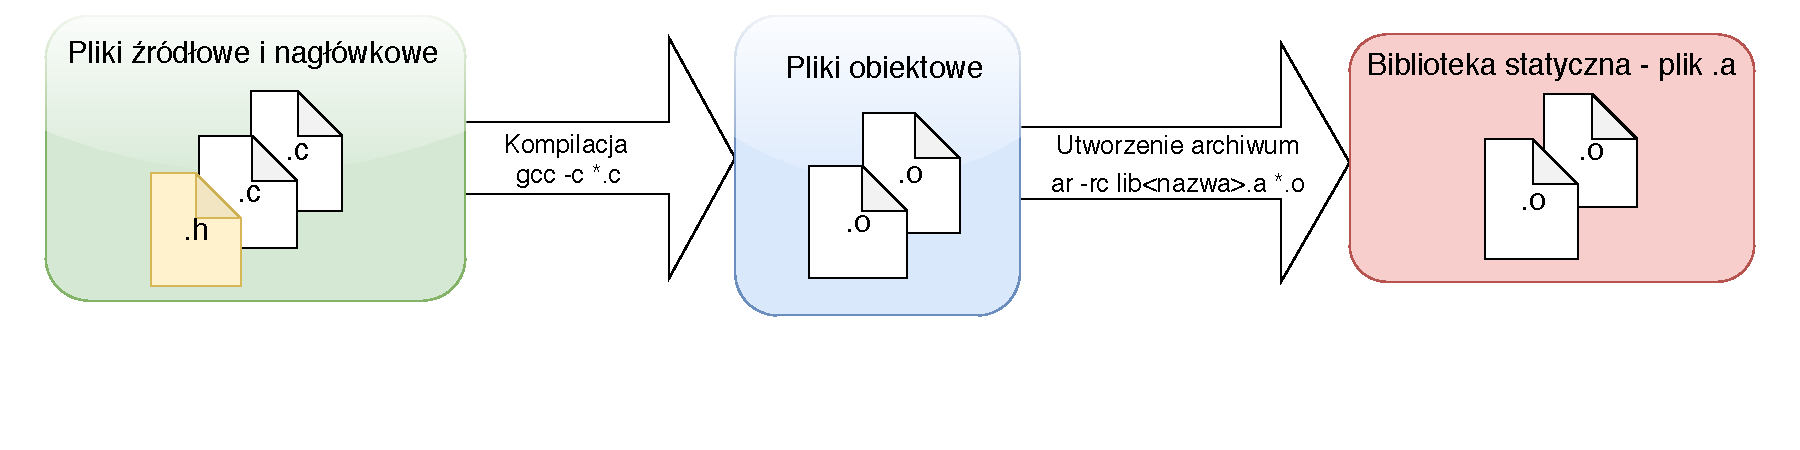
\includegraphics[width=\textwidth]{res/StaticLibFlow}
\end{figure}

Zawartość powstałego archiwum można zbadać za pomocą komendy \textit{ar -t} - wyświetla ona wszystkie pliki obiektowe wchodzące w~skład danej biblioteki. Istnieje również możliwość wypisania symboli - służy do tego narzędzie \textit{nm}. Użycie tych narzędzi na wykonanym przez autorów przykładzie ilustruje listing \ref{lst:libstat3}. Wynikiem polecenia \textit{nm} są tam dwa symbole, oznaczające dwie udostępnione dla użytkowników biblioteki funkcje (dodawanie i~odejmowanie liczb zespolonych).

\begin{lstlisting}[language=Cmd, caption={Użycie poleceń \textit{ar -t} oraz \textit{nm} na bibliotece statycznej.},label={lst:libstat3}]
user@host:~/complex$ ar -t libcoml.a
complex_opers.o
user@host:~/complex$ nm libcoml.a

complex_opers.o:
0000000000000000 T add_complex_numbers
0000000000000091 T subtract_complex_numbers
\end{lstlisting}

\newpage
\subsubsection*{Dołączanie utworzonej biblioteki do programu}
Rysunek \ref{fig:staticliblink} przedstawia schematycznie proces dołączania utworzonej biblioteki statycznej do programu. Proces ten składa się z~następujących etapów:

\begin{figure}[H]
\centering
\caption{Proces dołączania biblioteki statycznej do programu z~uwzględnieniem komend koniecznych do wykonania poszczególnych etapów \cite{Compiling}}
\label{fig:staticliblink}
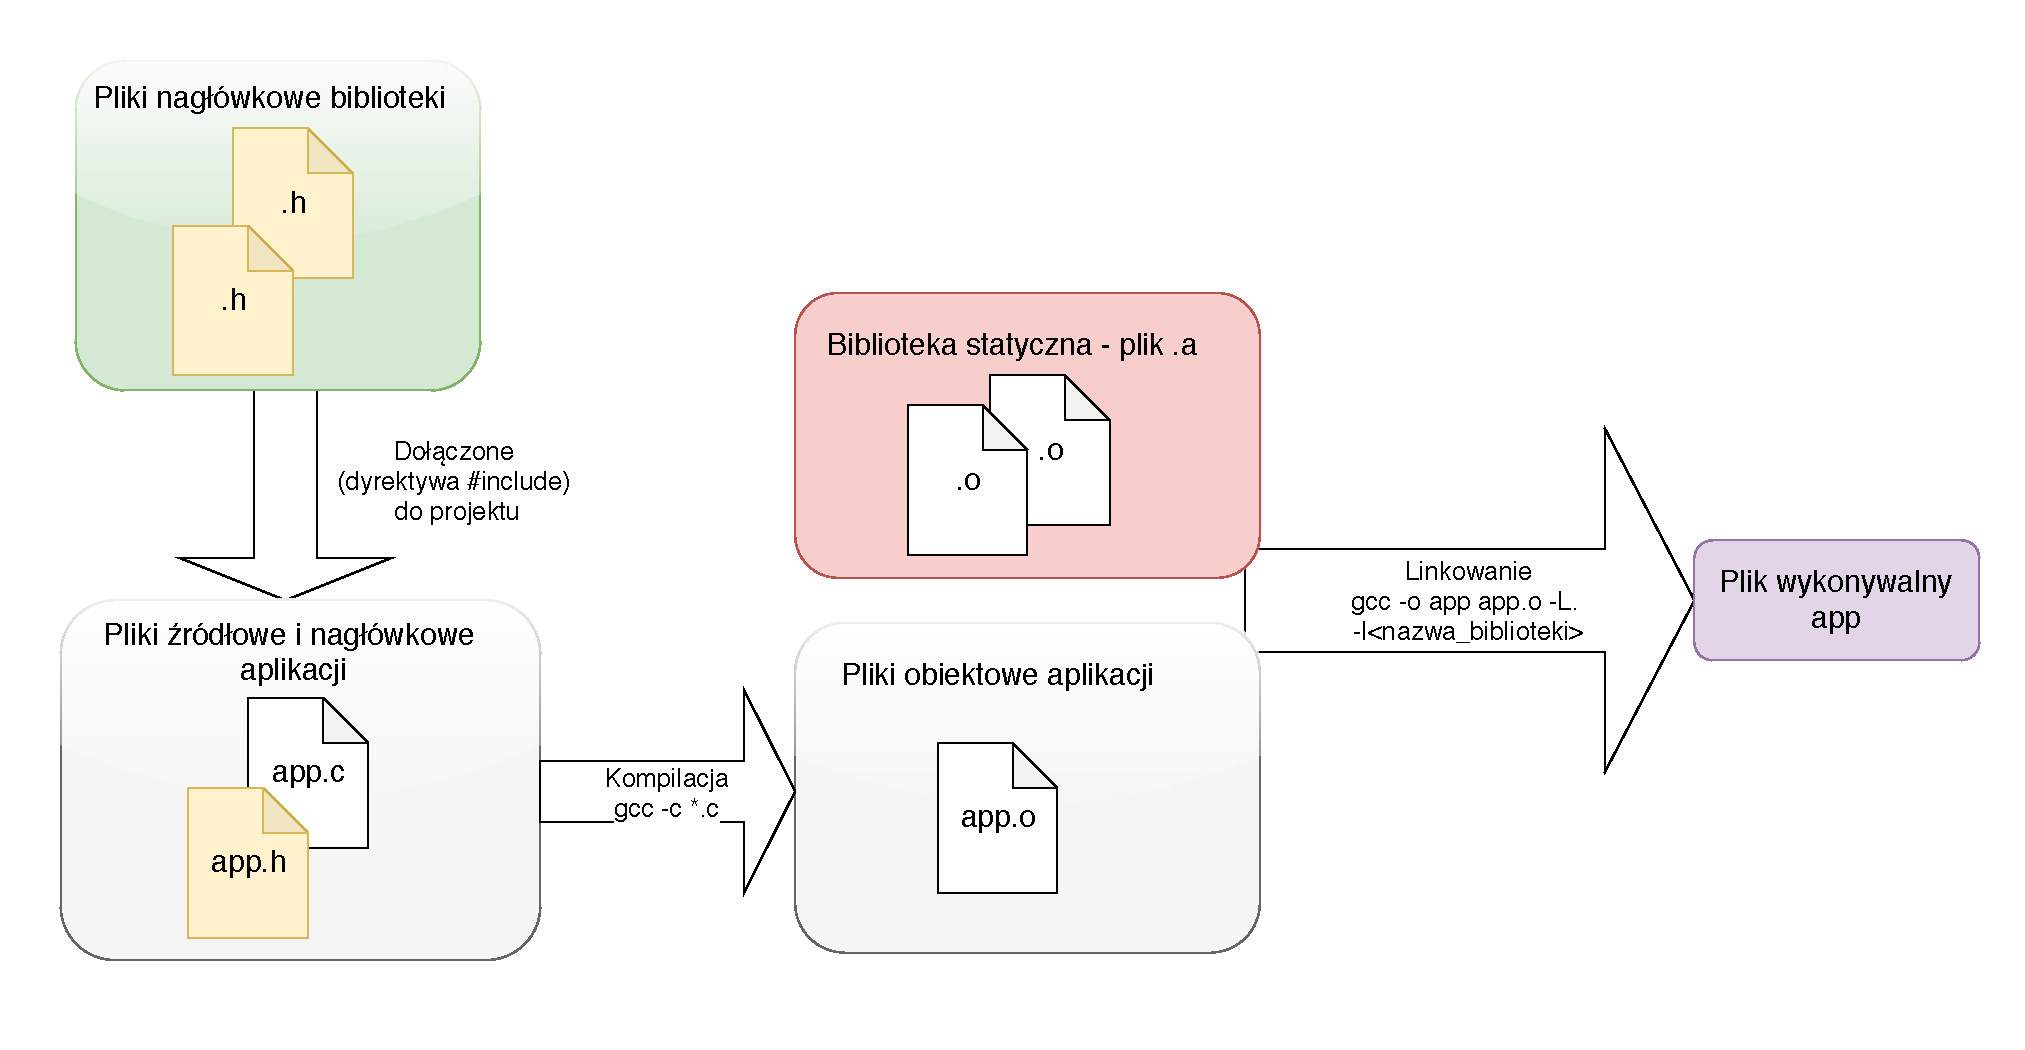
\includegraphics[width=\textwidth]{res/StaticLibLink}
\end{figure}

\begin{itemize}
\item dołączenie do źródeł programu plików nagłówkowych zawierających deklaracje stanowiące interfejs między programem a~biblioteką (dyrektywa \textit{include} - listing \ref{lst:libstat4}).

\begin{lstlisting}[language=c++, caption={Plik \textit{app.c} zawierający dyrektywę \textit{include} dołączającą plik nagłówkowy zawierający deklaracje funkcji z~biblioteki statycznej},label={lst:libstat4}]
#include "../complex/complex_opers.h"
#include <stdio.h>

int main(void) {

    complex_number a~= {2.5, 3.7};
    complex_number b = {3.5, 0};

    complex_number c = add_complex_numbers(a, b);
    complex_number d = subtract_complex_numbers(a, b);

    printf("%lf %lf\n", c.real, c.imaginary);
    printf("%lf %lf\n", d.real, d.imaginary);

    return 0;
}
\end{lstlisting}

\item kompilacja plików źródłowych programu do postaci plików obiektowych za pomocą \textit{gcc} (listing \ref{lst:libstat5}). Wynikiem powinien być zestaw plików obiektowych odpowiadający wykorzystanym plikom źródłowym.

\begin{lstlisting}[language=Cmd, caption={Kompilacja plików źródłowych głównego programu do postaci obiektowej.},label={lst:libstat5}]
user@host:~/app$ gcc -c *.c
user@host:~/app$ ls
app.c  app.o
\end{lstlisting}


\item połączenie plików obiektowych i~biblioteki w~plik wykonywalny za pomocą \textit{gcc} (listing \ref{lst:libstat6}). Opcja \textit{-L} pozwala określić ścieżkę do dołączanej biblioteki, natomiast \textit{-l} - nazwę biblioteki (bez przedrostka \textit{lib} i~rozszerzenie \textit{.a}).

\begin{lstlisting}[language=Cmd, caption={Linkowanie plików obiektowych programu z~biblioteką statyczną, wynik uruchomienia programu obrazuący poprawne działanie przykładu.},label={lst:libstat6}]
user@host:~/app$ gcc -o app app.o -L../complex -lcoml
user@host:~/app$ ls
app  app.c  app.o
user@host:~/app$ ./app
6.000000 3.700000
-1.000000 3.700000
\end{lstlisting}

\end{itemize}


%%%%%%%% BIBLIOTEKI DYNAMICZNE %%%%%%%%%%%%%%%%%%%%%%%%%%%%%%%%

\subsection{Biblioteki współdzielone}
Działanie bibliotek współdzielonych jest bardziej skomplikowane. Z~uwagi na fakt, iż w~projekcie GGSS biblioteki współdzielone są używane jedynie w~postaci zewnętrznych zależności, przedstawiony opis dotyczył będzie jedynie podstaw tworzenia i~działania tych bibliotek. Główna różnica w~stosunku do bibliotek statycznych polega na zmianie czasu, w~którym biblioteka jest dołączana do programu. W~przypadku bibliotek współdzielonych dzieje się to w~trakcie ładowania programu do pamięci. Oznacza to, że biblioteki te nie są częścią pliku wykonywalnego programu, dzięki czemu programy te mają mniejszy rozmiar i~nie ma konieczności ich ponownej kompilacji w~wypadku wprowadzenia zmian w~bibliotece. Ponadto kod bibliotek tego typu jest ładowany do pamięci tylko raz - przy pierwszym użyciu biblioteki, i~może być współdzielony. Podobnie jak wcześniej do tego typu bibliotek dołączone muszą być pliki nagłówkowe zawierające m.in. deklaracje funkcji stanowiących interfejs programistyczny pomiędzy biblioteką, a~używającym ją programem.

\newpage

\subsubsection*{Nazwy i~wersjonowanie bibliotek współdzielonych}
Podczas pracy z~bibliotekami współdzielonymi istotne jest przestrzeganie narzuconych konwencji dotyczących sposobu nadawania im nazw oraz ich wersjonowania. Rys. \ref{fig:sharedName} przedstawia poszczególne części składające się na poprawną nazwę pliku biblioteki. Składa się ona z~przedrostka \textit{lib}, po którym następuje właściwa nazwa biblioteki. Następnie po kropce powinno znaleźć się rozszerzenie \textit{.so} a~po nim, rozdzielone kropkami, liczby określające wersję biblioteki. 

\begin{figure}[H]
\centering
\caption{Elementy poprawnej nazwy biblioteki współdzielonej}
\label{fig:sharedName}
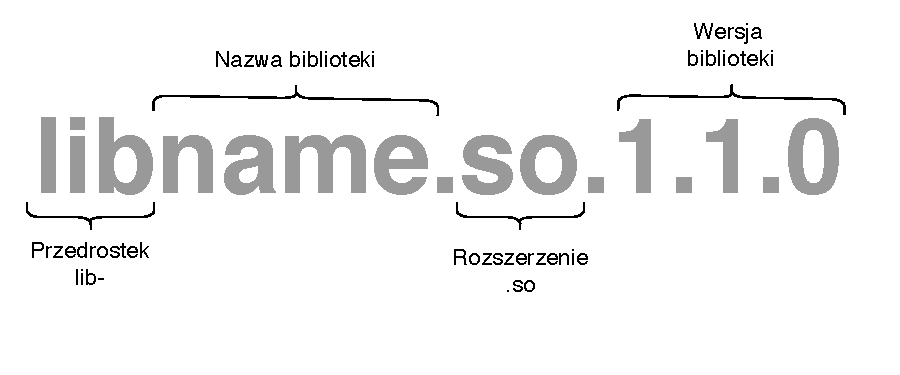
\includegraphics[width=\textwidth]{res/sharedLibName}
\end{figure}

Wersja biblioteki składa się z~trzech liczb \cite{TLDP}: 
\begin{itemize}
\item nadrzędny numer wersji (\textit{major version number}) - różnica na tym poziomie oznacza zmianę interfejsu skutkującą brakiem kompatybilności miedzy wersjami bibliotek
\item podrzędny numer wersji (\textit{minor version number}) - różnica na tym poziomie oznacza zwykle zachowaną kompatybilność między wersjami biblioteki
\item numer wydania (\textit{release number}) - opcjonalny
\end{itemize}

Poza nazwą samego pliku bibliotekę współdzieloną określają również dwie inne nazwy \cite{SharedNames}. Pierwsza z~nich to tzw. \textbf{soname}. Stanowi ona podzbiór nazwy przedstawionej na Rys. \ref{fig:sharedName}, bez dwóch ostatnich numerów wersji (przykład: \textit{libname.so.1}). Nazwa \textit{soname} stanowi zwykle nazwę dowiązania symbolicznego do pliku biblioteki. Druga z~nazw to tzw. \textbf{linker name} - stanowi ona nazwę biblioteki bez numeru wersji (tzn. np. \textit{libname.so}).


\subsubsection*{Tworzenie biblioteki współdzielonej}
Proces tworzenia biblioteki współdzielonej przedstawiony został na Rys. \ref{fig:sharedCreate}. Składa się on z~następujących etapów \cite{Shared1}:
\begin{itemize}
\item kompilacja plików źródłowych biblioteki do postaci obiektowej za pomocą \textit{gcc} (listing \ref{lst:socomp}). Konieczne jest zastosowanie flagi \textbf{-fPIC}, pozwalającej na wygenerowanie tzw. \textbf{Position Independent Code} - jest to taki kod maszynowy, który po załadowaniu do pamięci może być współdzielony przez kilka procesów. Wynikiem tej operacji są pliki obiektowe (\textit{*.o})

\begin{lstlisting}[language=bash, language=Cmd, caption={Kompilacja plików źródłowych biblioteki (zastosowanie flagi -fPIC)}, label={lst:socomp}]
user@host:~/complex$ gcc -fPIC -c *.c
user@host:~/complex$ ls
complex_number.h  complex_opers.c  complex_opers.h  complex_opers.o
\end{lstlisting}

\item utworzenie obiektu współdzielonego w~procesie linkowania (listing \ref{lst:socreation}). W~tym celu należy zastosować flagę \textbf{-shared}. Należy również przekazać do wynikowego pliku \textit{nazwę so (soname)}. Wartość pola \textit{SONAME} w~pliku biblioteki można następnie sprawdzić za pomocą narzędzia \textit{objdump} z~flagą \textit{-p}. Podobnie jak w~przypadku biblioteki statycznej możliwe jest również zbadanie występujących w~niej symboli za pomocą narzędzia \textit{nm} - z~uwagi na bardziej skomplikowaną naturę samego pliku ich lista jest jednak dłuższa. 

\begin{lstlisting}[language=bash, language=Cmd, caption={Utworzenie biblioteki współdzielonej, zbadanie wartości pola \textit{SONAME} w~utworzonym pliku}, label={lst:socreation}]
user@host:~/complex$ gcc -shared -Wl,-soname,libcoml.so.1 -o libcoml.so.1.0.0 *.o
user@host:~/complex$ ls
complex_number.h  complex_opers.c  complex_opers.h  complex_opers.o  libcoml.so.1.0.0
user@host:~/complex$ objdump -p libcoml.so.1.0.0 | grep SONAME
  SONAME               libcoml.so.1
\end{lstlisting}

\item utworzenie odpowiednich dowiązań symbolicznych. Istnieje kilka sposobów na linkowanie bibliotek współdzielonych. W~zależności od zastosowanego sposobu potrzebne mogą okazać się inne dowiązania. W~tym przypadku autorzy posłużyli się narzędziem \textbf{ldconfig} z~flagą \textit{-n} do wygenerowania dowiązania odpowiadającego nazwie \textit{soname} biblioteki (listing \ref{lst:ldconfig}).

\begin{lstlisting}[language=bash, language=Cmd, caption={Utworzenie dowiązania symbolicznego wskazującego na bibliotekę za pomocą programu \textit{ldcongfig}}, label={lst:ldconfig}]
user@host:~/complex$ ldconfig -n .
user@host:~/complex$ ls
complex_number.h  complex_opers.c  complex_opers.h  complex_opers.o  libcoml.so.1  libcoml.so.1.0.0
\end{lstlisting}

\end{itemize}

\begin{figure}[H]
\centering
\caption{Proces tworzenia biblioteki współdzielonej z~uwzględnieniem koniecznych poleceń \cite{Compiling}}
\label{fig:sharedCreate}
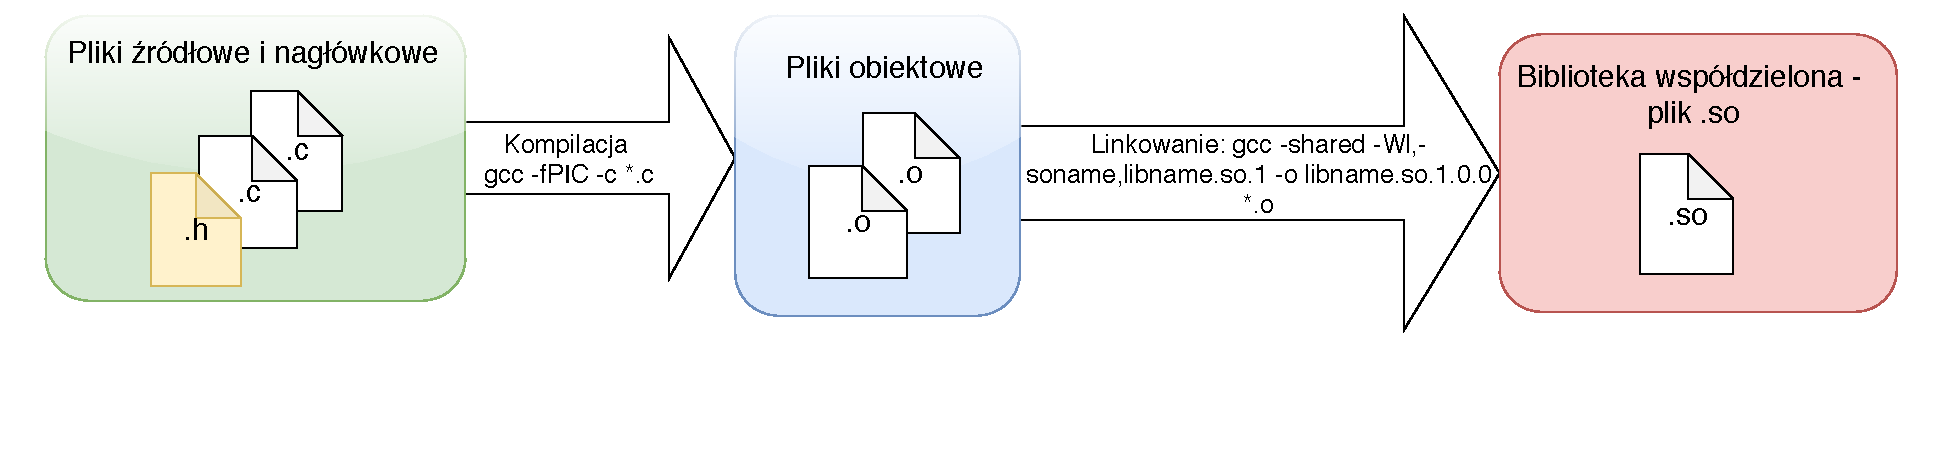
\includegraphics[width=\textwidth]{res/sharedLibFlow}
\end{figure}


\subsubsection*{Dołączanie utworzonej biblioteki do programu}
Proces dołączania utworzonej biblioteki współdzielonej do programu składa się z~następujących etapów:

\begin{itemize}
\item dołączenie do źródeł programu plików nagłówkowych zawierających deklaracje stanowiące interfejs między programem a~biblioteką (dyrektywa \textit{include}, identycznie jak w~przypadku biblioteki statycznej)

\item kompilacja plików źródłowych programu do postaci obiektowej (również analogicznie jak w~przypadku bibliotek statycznych)

\item linkowanie w~celu uzyskania pliku wykonywalnego (listing \ref{lst:sharedLinking}). W~zaprezentowanym przykładzie użyte zostało stworzone wcześniej dowiązanie symboliczne \textit{libcoml.so.1}.

\begin{lstlisting}[language=bash, language=Cmd, caption={Linkowanie w~celu uzyskania pliku wykonywalnego zależnego od biblioteki współdzielonej}, label={lst:sharedLinking}]
user@host:~/app$ gcc -o app app.o -L../complex -l:libcoml.so.1
user@host:~/app$  ls
app  app.c  app.o
\end{lstlisting}

\end{itemize}

Istnieje możliwość wyświetlenia, od jakich bibliotek współdzielonych jest zależny dany plik wykonywalny. Można to osiągnąć za pomocą narzędzie \textbf{ldd} \cite{shared2}, co zostało ukazane na listingu \ref{lst:sharedFailed}. Aktualnie stworzona przez autorów biblioteka jest oznaczona jako nie znaleziona (\textit{not found}). Z~tego też powodu próba uruchomienia programu zakończy się porażką. 

\newpage

\begin{lstlisting}[language=bash, language=Cmd, caption={Użycie polecenia \textit{ldd} i~pierwsza, nieudana próba uruchomienia aplikacji zależnej od biblioteki współdzielonej}, label={lst:sharedFailed}]
user@host:~/app$ ldd app
        linux-vdso.so.1 (0x00007fffc16b6000)
        libcoml.so.1 => not found
        libc.so.6 => /lib/x86_64-linux-gnu/libc.so.6 (0x00007f3e5e8b0000)
        /lib64/ld-linux-x86-64.so.2 (0x00007f3e5f000000)
user@host:~/app$ ./app
./app: error while loading shared libraries: libcoml.so.1: cannot open shared object file: No such file or directory
\end{lstlisting}

\subsubsection*{Uruchamianie programu zależnego od biblioteki współdzielonej}
Poprzednia próba uruchomienia biblioteki zakończyła się porażką. Wynika to z~tego, że program \textbf{loader} (linker dynamiczny) nie zna ścieżki, pod którą powinien znaleźć bibliotekę. Jednym z~rozwiązań tego problemu jest dodanie tej ścieżki do zmiennej środowiskowej \textbf{LD\_LIBRARY\_PATH} \cite{shared3}. Odpowiednie polecenie oraz poprawne uruchomienie programu ilustruje listing \ref{lst:sharedOK}.

\begin{lstlisting}[language=bash, language=Cmd, caption={Dodanie ścieżki zawierającej bibliotekę do zmiennej \textit{LD\_LIBRARY\_PATH} i~poprawne uruchomienie przykładowej aplikacji}, label={lst:sharedOK}]
user@host:~/complex$ export LD_LIBRARY_PATH=$(pwd):$LD_LIBRARY_PATH
user@host:~/complex$ cd ../app/
user@host:~/app$ ./app
6.000000 3.700000
-1.000000 3.700000
\end{lstlisting}

%%%%%%%%%%%%%%%%%%%% KONIEC BIBLIOTEK %%%%%%%%%%%%%%%%%%%%%%%%%%%%%%%%%%%%

\section{Narzędzie CMake}

\textit{CMake (Cross-platform Make)} to narzędzie pozwalające na konfigurację procesu budowania oprogramowania (aplikacji oraz bibliotek) w~sposób niezależny od platformy. Jego działanie opiera się na generowaniu pliku budującego natywnego dla określonej platformy \cite{CMakeIntro} (dla systemów z~rodziny UNIX jest nim \textit{Makefile}) na podstawie przygotowanego przez użytkownika pliku \textit{CMakeLists.txt}. Takie podejście w~znacznym stopniu ułatwia tworzenie aplikacji multiplatformowych oraz pozwala na intuicyjne zarządzanie zależnościami w~projekcie. Domyślnie CMake pracuje z~językami C i~C++, natomiast nowe wersje narzędzia wpierają ponadto m.in. język C\# czy technologię CUDA \cite{CMakeSupport}. Narzędzie to jest rozwijane i~wspierane przez firmę \textit{Kitware}.\par

\subsubsection*{Plik CMakeLists.txt}
Jak wspomniano wyżej działanie narzędzia CMake opiera się na przygotowanym przez użytkownika pliku (lub zestawie plików rozmieszczonych w~strukturze katalogów projektu) \textit{CMakeLists.txt}. Plik ten zawiera polecenia napisane w~specjalnie do tego celu przygotowanym języku skryptowym. Użytkownik może za jego pomocą  m.in. określać jakie pliki wykonywalne mają zostać wygenerowane podczas procesu budowania, wskazać lokalizację plików źródłowych czy określić zależności między komponentami projektu oraz bibliotekami zewnętrznymi. \par

\subsubsection*{Prosty przykład}
Listing \ref{lst:hello} zawiera przykład prostego pliku \textit{CMakeLists.txt}, pozwalającego na zbudowanie napisanej w~języku C++ obiektowej wersji klasycznego programu \textit{Hello world}. Przykład ilustruje zastosowanie podstawowych poleceń CMake do określenia minimalnej wersji narzędzia, standardu języka C++, wynikowego pliku wykonywalnego oraz potrzebnych plików nagłówkowych. \par

\begin{lstlisting}[language=cmake,caption={Przykład prostego pliku CMakeLists.txt przeznaczonego do budowania programu napisanego w~C++}, label={lst:hello}]
# Określenie minimalnej wersji CMake
cmake_minimum_required(VERSION 3.0 FATAL_ERROR)

# Określenie standardu języka C++
set(CMAKE_CXX_STANDARD 14)
set(CMAKE_CXX_STANDARD_REQUIRED True)

# Nazwa oraz wersja projektu
project(Hello VERSION 1.0)

# Dodanie pliku wykonywalnego, który powinien powstać
# wskutek procesu budowania
add_executable(Hello Main.cpp)

# Dodanie do projektu katalogu include wraz ze znajdującym się 
# wewnątrz niego plikiem nagłówkowym
target_include_directories(Hello PUBLIC "${CMAKE_CURRENT_SOURCE_DIR}/include")
\end{lstlisting}

\subsubsection*{Wersje CMake}
CMake jest narzędziem, który w~ciągu ostatnich kilku lat przechodzi gruntowne zmiany. Starsze wersje (np. 2.8) oparte są o~prosty system zmiennych \cite{CMakeRight}, co wprowadza szereg trudności w~zarządzaniu dużymi projektami z~wielopoziomowymi drzewami zależności. Dodatkowym problemem tych wersji jest również brak dobrze zdefiniowanych tzw. \textit{dobrych praktyk} oraz nieprzystępna dla początkujących dokumentacja. Współczesne wersje narzędzie CMake (zwykle za takie uznaje się nowsze od wersji 3.0) opierają się na innym  podejściu, opartym na strukturze projektu \cite{CMakeRight}, co było przyczyną pojawienia się dla nich wyżej wspomnianych \textit{dobrych praktyk}. Zalecane jest więc, by nowe projekty prowadzone były właśnie z~użyciem nowszych wersji narzędzia.

\subsubsection*{Narzędzia CTest i~CPack}
CMake oferuje również możliwość konfiguracji sposobu testowania projektu. Służy do tego narzędzie \textit{CTest}, dystrybuowane razem z~podstawowym narzędziem CMake. Innym przydatnym modułem jest \textit{CPack} - narzędzie to służy przygotowywaniu pakietów instalacyjnych z~oprogramowaniem. Użycie obu wymienionych narzędzi polega na umieszczeniu w~pliku \textit{CMakeLists.txt} kilku przeznaczonych do tego komend. \par 


\section{Język Python}
\textit{Python} jest nowoczesnym, wysokopoziomowym językiem programowania, wspierającym takie paradygmaty jak programowanie obiektowe czy imperatywne. Działanie Pythona opiera się na dynamicznym systemie typów. Z~założenia Python jest językiem przyjemnym w~użytkowaniu, co przyczyniło się do jego dużej popularności \cite{Lutz}. Python jest szeroko stosowany jako język skryptowy - takie też zastosowanie znalazł w~projekcie GGSS.

\subsubsection*{Prosty przykład}
Listing \ref{lst:pyexample} przedstawia prosty przykład skryptu napisanego w~języku Python w~wersji 3. Kod ten stanowi uproszczoną wersję skryptu zaprezentowanego w~dalszej części pracy, którego zadaniem jest zbudowanie aplikacji w~zależności od przekazanych przez użytkownika argumentów. Przykład prezentuje prosty skrypt przyjmujący jeden z~dwóch możliwych argumentów i~wypisujący informację na temat otrzymanego argumentu na standardowe wyjście.

\begin{lstlisting}[language=python,caption={Przykład prostego skryptu napisanego w~języku Python 3 - przetwarzanie argumentów podanych przez użytkownika do skryptu}, label={lst:pyexample}]
import argparse

## Prosty skrypt przetwarzający argumenty podane 
## przy jego uruchomieniu przez użytkownika

## Definicja funkcji w~języku Python
def parse_command_line_arguments():

    ## Obiekt przetwarzający argumenty (parser)
    parser = argparse.ArgumentParser()

    ## Argumenty wzajemnie się wykluczające
    group = parser.add_mutually_exclusive_group(required=True)
    group.add_argument("-s", "--staticboost", 
        help="Use static Boost linking.", action="store_true")
    group.add_argument("-d", "--dynamicboost",
        help="Use dynamic Boost linking.", action="store_true")

    return parser.parse_args()

if __name__=="__main__":
    ## Wywołanie funkcji
    arguments = parse_command_line_arguments()
    print(arguments)


\end{lstlisting}

\subsubsection*{Wersje języka Python}
Python funkcjonuje w~dwóch wersjach: Python 2 oraz 3. Wersje te nie są ze sobą w~pełni kompatybilne, tzn. pewne funkcjonalności Pythona 2 nie są dostępne w~Pythonie 3 i~odwrotnie. Różnice znaleźć można również np. w~domyślnym sposobie kodowania łańcuchów znakowych (ASCII w~Pythonie 2, Unicode w~Pythonie 3) oraz w~wyniku dzielenia (za pomocą operatora \textit{/}) dwóch liczb całkowitych (w Pythonie 2 wynikiem jest liczba całkowita, w~Pythonie 3 liczba zmiennoprzecinkowa typu \textit{float}) \cite{Python2vs3}. Ponadto zakończenie oficjalnego wsparcia Pythona w~wersji 2 przewidziane jest na styczeń 2020 roku \cite{Python2Countdown} - co w~momencie pisania niniejszej pracy (grudzień 2019) jest terminem niedalekim i~miało kluczowe znaczenie w~czasie podejmowania pewnych decyzji projektowych.

\subsubsection*{Zewnętrzne biblioteki}
Jedną z~największych zalet Pythona jest bardzo duża liczba bibliotek zewnętrznych tworzonych przez społeczność Pythona. Rozbudowują one język o~wiele nowych funkcjonalności, np. przetwarzanie plików HTML czy wykonywanie obliczeń numerycznych. W~niniejszej pracy zastosowanych zostało kilka tego typu bibliotek, m.in. \textit{Beautiful Soup} do wspomnianego wyżej przetwarzania dokumentów w~formacie HTML. Omówienie ich działania na przykładach znaleźć można w~dalszej części pracy - przy opisie konkretnego ich zastosowania. 


\section{Powłoka systemu operacyjnego (Bash)}
Powłoka systemu jest programem, którego głównym zadaniem jest udostępnienie interfejsu umożliwiającego łatwy dostęp do funkcji systemu operacyjnego. Nazwę \textit{powłoka} zawdzięcza temu, że jest warstwą okalającą system operacyjny. Najczęściej spotykanym rodzajem powłoki są tzw. interfejsy z~wierszem poleceń (ang. command-line interface). Polecenia wprowadzane są do nich w~modzie interaktywnym, tj. wykonywane są one w~momencie wprowadzenia końca linii.

\begin{lstlisting}[language=bash,language=Cmd,caption={Komenda wypisująca tekst na standardowe wyjście wykonana z~linii poleceń}]
user@host:~$ echo "interfejs z~linią poleceń"
interfejs z~linią poleceń
user@host:~$
\end{lstlisting}

Bash, czyli \textbf{Bourne Again Shell} jest powłoką systemu początkowo napisaną dla systemu operacyjnego GNU. Obecnie Bash jest kompatybilny z~większością systemów Unixowych, gdzie zwykle jest powłoką domyślną oraz posiada kilka portów na inne platformy, tj.: MS-DOS, OS/2, Windows \cite{BashMan}. Oprócz pełnienia wyżej wymienionej funkcji, Bash jest również językiem programowania pozwalającym na tworzenie skryptów, które są kolejną metodą wprowadzania poleceń do powłoki systemu.\par
Korzystając z~języka skryptowego powłoki Bash jesteśmy w~stanie zawrzeć dodatkową logikę podczas wykonywania komend. Wspiera on takie struktury jak: instrukcje warunkowe, pętle, operacje logiczne oraz arytmetyczne. Aby wykorzystać Bash w~skrypcie należy na początku pliku zamieścić zapis \textbf{\#!/bin/bash}, gdzie \textbf{/bin/bash} to ścieżka do pliku interpretera Bash. Zachowanie skryptu jesteśmy w~stanie uzależnić od argumentów wykonania. Ich obsługa odbywa się za pomocą zapisu \textbf{\$?}, gdzie \textbf{?} jest to numer porządkowy argumentu liczony od 0.

\begin{lstlisting}[label={lst:prostySkrypt},language=bash,caption={Skrypt wykorzystujący argumenty wejściowe, instrukcję warunkową oraz polecenie echo}]
#!/bin/bash
if [ $1 == "argumenty" ]; then
        echo "Argument 0.: $0"
        echo "Argument 1.: $1"
else
        echo "Nieznane polecenie"
fi
\end{lstlisting}

\begin{lstlisting}[language=bash,language=Cmd,caption={Przykład działania Skryptu z~Listingu \ref{lst:prostySkrypt}}]
user@host:~$ /home/user/prostySkrypt.sh argumenty
Argument 0.: /home/user/prostySkrypt.sh
Argument 1.: argumenty
\end{lstlisting}

Bash posiada wiele poleceń, które pozwalają na wykonywanie zarówno podstawowych, jak i~bardziej zaawansowanych czynności, np.: obsługa plików, obsługa systemu katalogów, zarządzanie kontami, uprawnieniami, itd.\par
Bash posiada również wiele zaawansowanych funkcjonalności, które pozwalają na kontrolowanie przepływu informacji w~trakcie wykonywania poleceń. Przykładem jest wpisywanie tekstu do pliku ukazane na Listingu \ref{lis:zapisDoPliku}.

\begin{lstlisting}[label={lis:zapisDoPliku},language=Cmd,caption={Przykład zapisu tekstu do pliku}]
user@host:~$ echo "Ten napis zostanie zapisany do pliku plik.txt" > plik.txt
user@host:~$ cat plik.txt
Ten napis zostanie zapisany do pliku plik.txt
\end{lstlisting}

W celu zapisania tekstu do pliku należy na standardowe wyjście przekazać napis za pomocą komendy \textbf{echo}, a~następnie przekierować za pomocą zapisu \textbf{>}, który poprzedza nazwę pliku docelowego. W~wyniku działania zawartość pliku \textbf{plik.txt} zostanie nadpisana, a~w przypadku gdy takiego pliku nie ma, to zostanie on utworzony i~uzupełniony o~napis.\par


\section{System kontroli wersji Git i~portal Gitlab}
System kontroli wersji Git jest oprogramowaniem służącym do śledzenia i~zarządzania zmianami w~plikach projektowych. W~przypadku Git'a, aby zarejestrować pliki projektowe w~celu ich śledzenia należy wykonać kilka czynności. Po pierwsze wymagane jest utworzenie repozytorium. Sprowadza się ono do wykonania odpowiedniej komendy Git'a wewnątrz folderu projektu, tj. \textbf{git init}. Podczas działania komendy wewnątrz folderu, w~którym wywołaliśmy ww. polecenie, inicjowany jest ukryty folder \textbf{.git}
. Jest on odpowiedzialny za przechowywanie konfiguracji dla tego repozytorium oraz zapisywanie informacji o~wszystkich zmianach dokonanych w~projekcie.

\begin{lstlisting}[language=bash,language=Cmd,caption={Inicjalizacja repozytorium git}]
user@host:/ścieżka/do/projektu$ git init
Initialized empty Git repository in /ściezka/do/projektu
user@host:/ściezka/do/projektu$ ls .git
branches  config  description  HEAD  hooks  info  objects  refs
\end{lstlisting}

Taka inicjalizacja nie spowoduje żadnego dodatkowego działania oprócz utworzenia repozytorium. Żadne pliki nie są jeszcze poddawane rewizji. W~celu rejestracji plików należy wykonać jeszcze kilka kroków. Pierwszym z~nich jest wykonanie komendy \textbf{git add}, która poprzedza nazwę plików lub folderów, które chcemy poddać wersjonowaniu. Elementy te zostają dodane do tzw. poczekalni, czyli są one kandydatami do utworzenia kolejnej rewizji. Przydatną komendą w~tym przypadku jest również \textbf{git status} pozwalająca na sprawdzenie obecnego stanu repozytorium. Wyświetla ono krótkie podsumowanie nt. nowych plików, usuniętych plików oraz plików zmodyfikowanych. Informuje nas również o~tym, które pliki są brane pod uwagę do utworzenia kolejnej rewizji.

%% Jesli chcemy uzywac mojego stylu, musimy miec konsystentnie $ albo # na koncu command-prompt
\begin{lstlisting}[language=Cmd,caption={Dodawanie elementów do poczekalni}]
user@host:/ściezka/do/projektu$ git add plik1 folder1
user@host:/ściezka/do/projektu$ git status
On branch master

No commits yet

Changes to be committed:
  (use "git rm --cached <file>..." to unstage)

        new file:   folder1/plik3
        new file:   folder1/plik4
        new file:   plik1

Untracked files:
  (use "git add <file>..." to include in what will be committed)

        plik2
\end{lstlisting}

\begin{figure}[H]
\centering
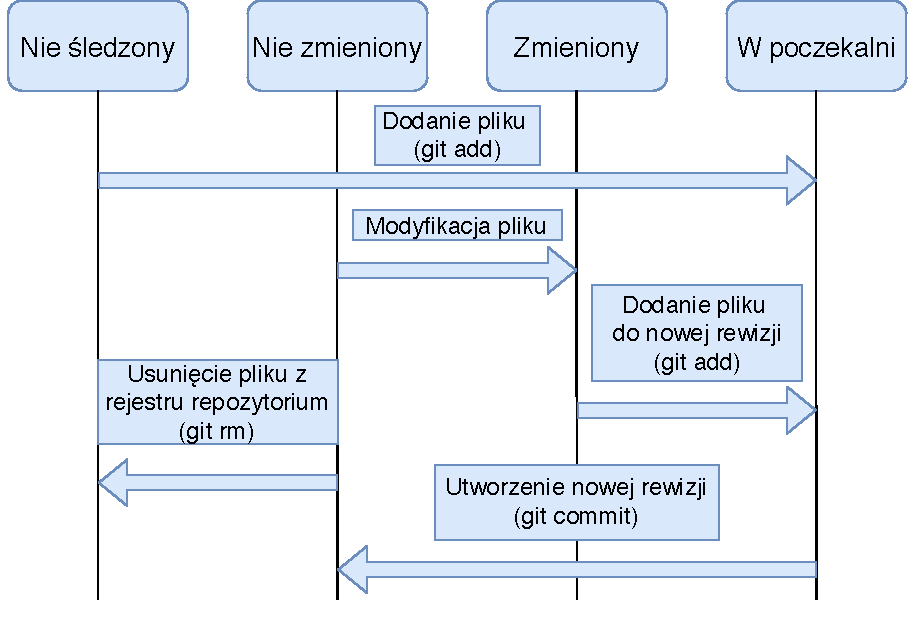
\includegraphics[width=0.8\textwidth]{res/fileStates.pdf}
\caption{Możliwe stany pliku w~repozytorium \cite{GitChart}} 
\end{figure}

Tworzenie nowej wersji w~ramach repozytorium odbywa się za pomocą komendy \textbf{git commit}. Sprowadza się do 'zamrożenia' obecnych wersji plików zarejestrowanych do rewizji oraz przypisanie im wspólnego, unikalnego dla każdej z~nich, identyfikatora. Git udostępnia komendy pozwalające na przeglądanie oraz przywracanie plików do wcześniej utworzonych wersji. Listing \ref{lis:pierwszaRewizja} przedstawia utworzenie nowej wersji oraz wyświetlenie podsumowania o~utworzonych do tej pory rewizjach.

\begin{lstlisting}[label={lis:pierwszaRewizja}, language=Cmd,caption={Utworzenie nowej rewizji}]
user@host:/sciezka/do/projektu$ git commit -m "Pierwsza rewizja"
user@host:/sciezka/do/projektu$ git log 
commit 1d2445e961beb25940dffa9d73963f887ee553ad
Author: user <user@localdomain>
Date:   Wed Dec 4 17:29:55 2019 +0100

    Pierwsza rewizja
\end{lstlisting}

Przejścia między rewizjami nie powodują utraty danych, gdyż zachowywana jest informacja o~stanie plików dla każdej z~nich, co ukazuje Listing \ref{lis:drugaRewizja}. Tworzona jest nowa rewizja zawierająca dodatkowo \textbf{plik2}, natomiast po powrocie do poprzedniej wersji plik ten nie występuje. Gdy powrócimy do nowszej wersji ponownie pojawi się \textbf{plik2}.

\begin{lstlisting}[language=Cmd,caption={Podsumowanie rewizji, powrót do starszej wersji},label={lis:drugaRewizja}]
user@host:/sciezka/do/projektu$ git add plik2
user@host:/sciezka/do/projektu$ git commit -m "Druga rewizja"
user@host:/sciezka/do/projektu$ git log 
commit b58836df55fc2a8eb2a43aa96273853776924807
Author: user <user@localdomain>
Date:   Wed Dec 4 17:30:10 2019 +0100

    Druga rewizja

commit 1d2445e961beb25940dffa9d73963f887ee553ad
Author: user <user@localdomain>
Date:   Wed Dec 4 17:29:55 2019 +0100

    Pierwsza rewizja

user@host:/sciezka/do/projektu$ ls
folder1  plik1  plik2
user@host:/sciezka/do/projektu$ git checkout 1d2445e961beb25940dffa9d73963f887ee553ad
user@host:/sciezka/do/projektu$ ls
folder1  plik1
user@host:/sciezka/do/projektu$ git checkout b58836df55fc2a8eb2a43aa96273853776924807
user@host:/sciezka/do/projektu$ ls
folder1  plik1  plik2
\end{lstlisting}

Głównym celem portalu \textbf{GitLab} jest udostępnienie środowiska do przechowywania repozytoriów Gitowych na zdalnych serwerach. Pozwala to na uniezależnienie się od maszyny na której pracujemy, zwiększa bezpieczeństwo plików źródłowych poprzez umieszczenie kopii na zdalnym serwerze oraz wspiera zespołową pracę nad kodem.\par

Ze względu na to, że portale typu \textbf{GitLab} są traktowane jako podstawowe narzędzie do wspólnej pracy nad kodem, to rozwinęły one wiele narzędzi wspomagających organizację oraz śledzenie pracy. Oprócz ww. funkcji \textbf{Gitlab} dostarcza wiele narzędzi do wspomagania procesu zapewniania jakości, jak i~automatyzacji dostarczania kodu.\par

\textbf{Git} posiada specjalne komendy pozwalające na przekazywanie oraz pobieranie repozytoriów z~ww. portali, czyli:
\begin{itemize}
\item \textbf{git clone}, która pozwala na pobranie repozytorium z~portalu oraz zainicjalizowanie go lokalnie
\item \textbf{git pull} - za pomocą tej komendy możemy zaktualizować repozytorium lokalne do najnowszej rewizji, która znajduje się na portalu
\item oraz komenda \textbf{git push} aktualizująca zdalne repozytorium do najnowszej lokalnej wersji
\end{itemize}

Bardzo ważnym aspektem technologii \textbf{GIT} jest mechanizm gałęzi (ang. \textit{branch}). Pozwala on na równoległą pracę nad jedną częścią kodu. Polega to na tym, że w~momencie utworzenia nowej gałęzi tworzymy tak na prawdę osobny łańcuch rewizji, których jedyną wspólną częścią jest rewizja wzorcowa, czyli wersja na podstawie której została utworzona gałąź, co przedstawia Rysunek \ref{fig:branch}. W~celu utworzenia nowej gałęzi należy wykorzystać komendę \textbf{git branch <nazwa-gałęzi>}, a~w celu zmiany aktualnie używanej gałęzi \textbf{git checkout <nazwa-gałęzi>}. Główna gałąź projektu nazywa się \textbf{master}. Zmiany na jednej gałęzi nie wpływają w~żaden sposób na inną gałąź do momentu tzw. \textbf{merge}, czyli złączenia dwóch gałęzi. Ważnym aspektem łączenia gałęzi jest rozwiązywanie konfliktów, które pojawiają się w~momencie, gdy łączone gałęzie wprowadzały zmiany do tego samego pliku, a~system rozwiązujący konflikty nie był w~stanie wykonać swojego zadania automatyczne. W~takim przypadku wymagana jest akcja programisty, aby w~gałęzi wynikowej zachować odpowiedni kod.

\begin{figure} [H]
\centering
\caption{Schemat tworzenia rewizja w~ramach nowej gałęzi}
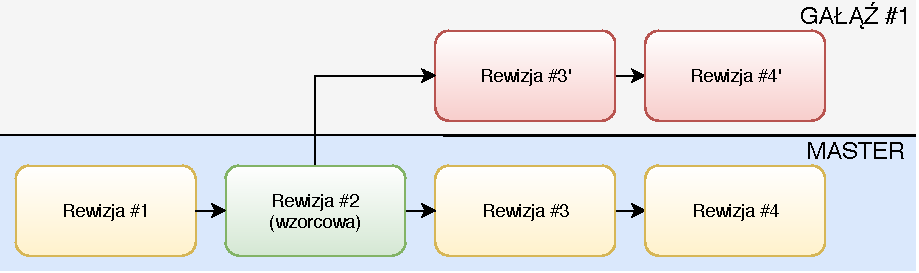
\includegraphics[width=\textwidth]{res/branch}
\label{fig:branch}
\end{figure}

\begin{figure} [H]
\centering
\caption{Schemat złączania gałęzi w~ramach polecenie \textbf{git merge}}
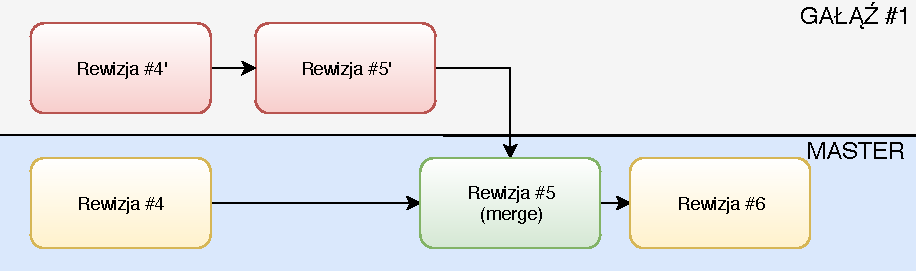
\includegraphics[width=\textwidth]{res/branchMerge}
\label{fig:branch}
\end{figure}

Jest to tylko podstawowy opis technologii jaką jest \textbf{Git}, przykłady bardziej zaawansowanych zastosowań pojawią się w~części manuskryptu przeznaczonej na prezentację wykonanych prac w~ramach projektu.


\section{Menadżer pakietów RPM}
Menadżer pakietów jest zbiorem oprogramowania, które w~sposób automatyczny zarządza instalacją, aktualizacją, konfiguracją oraz usuwaniem programów komputerowych \cite{ManagerWiki}. Ze względu na to, że procesy te różnią się w~zależności od systemów operacyjnych oraz ich dystrybucji istnieje wiele menadżerów pakietów.\par

Zastosowanie technologii zarządzania pakietami pozwala znacząco zmniejszyć próg wejścia wynikający z~użycia wcześniej niewykorzystywanego oprogramowania. Pozwala on odejść od żmudnego procesu ręcznej instalacji zależności oraz konfiguracji środowiska. Dzięki menadżerom wszystko jest wykonywane automatycznie. Jeżeli w~trakcie procedur nie wystąpi żaden problem, to pakiet, którego zleciliśmy instalacje, powinien być od razu gotowy do działania. Jeżeli domyślna konfiguracja, jaka zostanie nam zapewniona w~podczas działania menadżera pakietów, nie będzie dla nas odpowiednia możemy dokonać jej modyfikacji po procesie instalacji.

RPM, czyli RedHat Package Manager jest darmowym, open-source'owym menadżerem pakietów dla systemów z~rodziny RedHat oraz SUSE, czyli m.in.:
\begin{itemize}
\item RedHat Linux
\item CentOS
\item Fedora
\item openSUSE
\end{itemize}\par
RPM jest domyślnym menadżerem pakietów dla ww. dystrybucji. Obsługuje on pakiety w~ramach formatu \textbf{.rpm}. Pakiety \textbf{.rpm} zawierają w~sobie wiele ważnych elementów. Po pierwsze wewnątrz nich przechowywane są dane aplikacji, czyli: pliki wykonywalne, dokumentacja, testy, konfiguracja.\par 
Kolejnym ważnym elementem są informacje o~zależnościach, czyli innych wymaganych pakietach, które pozwalają na automatyzację procesu instalacji. W~momencie, gdy któraś z~zależności jest niespełniona menadżer pakietów stara się odnaleźć, w~bazie danych pakietów, odpowiedni wpis, aby \textbf{pobrać} oraz \textbf{zainstalować} brakujące oprogramowanie. Trzecim ważnym elementem jest logika pakietu, która jest podstawą do realizacji akcji wykonywanych przez menadżer pakietów, dostarczona w~postaci skryptów powłoki, np. \textbf{bash}, zaszytych wewnątrz pliku *.rpm.

Listing \ref{lst:zawRPM} pokazuje przykładową zawartość pakietu, czyli moduł kernela \textbf{modułAplikacji}, plik w~formacie \textbf{JSON} pozwalający na konfigurację aplikacji oraz plik wykonywalny \textbf{aplikacji}, natomiast  listing \ref{lst:skryptRPM} pokazuje przykładową logikę pakietu RPM w~postaci skryptów shell. Skrypty te nie zawierają ani kopiowania, ani usuwania plików zawartych pakiecie, proces ten odbywa się automatycznie na podstawie ścieżek ukazanych na Listingu \ref{lst:zawRPM} w~trakcie instalacji/dezinstalacji.

\begin{lstlisting}[language=Cmd,caption={Przykładowa zawartość pakietu RPM},label={lst:zawRPM}]
user@host:~$ rpm -qpl pakiet.rpm
/ścieżka
/ścieżka/do
/ścieżka/do/konfiguracjaAplikacji.json
/ścieżka/do/aplikacji
/usr
/usr/lib
/usr/lib/modules
/usr/lib/modules/3.10.0-862
/usr/lib/modules/3.10.0-862/extra
/usr/lib/modules/3.10.0-862/extra/modułAplikacji.ko
\end{lstlisting}

\begin{lstlisting}[label={lst:skryptRPM}, language=Cmd, caption={Skrypty pakietu RPM}]
user@host:~$ rpm -qp --scripts pakiet.rpm
preinstall program: /bin/sh
postinstall scriptlet (using /bin/sh):

#!/bin/sh
echo "Post-instajacja przykładowego pakietu"
echo "Przypisywanie uprawnień"
chmod 777 /ścieżka/do/konfiguracjaAplikacji.json
echo "Ładowanie modułu aplikacji"
/sbin/modrpobe modułAplikacji

preuninstall scriptlet (using /bin/sh):
#!/bin/sh
echo "Odinstalowywanie przykładowego pakietu"
echo "Usuwanie modułu aplikacji"
/sbin/rmmod modułAplikacji

postuninstall program: /bin/sh
\end{lstlisting}

\section{Technologie wirtualizacji i~konteneryzacji}

\textbf{Wirtualizacja}, czyli proces uruchamiania instancji wirtualnego systemu komputerowego odseparowanego od rzeczywistego systemu komputerowego oraz jego sprzętu (ang. hardware). Pozwala na uruchomienie \textbf{wielu różnych} systemów operacyjnych na jednym komputerze \textbf{jednocześnie}. Wykorzystywany przede wszystkim do separacji środowisk dla aplikacji, czy też całych systemów. Pozwala na uruchomienie oprogramowania nieprzystosowanego do naszego systemu operacyjnego, wystarczy utworzyć instancję maszyny wirtualnej z~odpowiednim systemem operacyjnym. Aplikacje uruchamiane w~takiej instancji zachowują się tak, jakby znajdowały się na \textbf{odseparowanym komputerze} z~własnym, dedykowanym systemem operacyjnym, bibliotekami oraz innym oprogramowaniem. Dużym plusem jest pełna separacja instancji uruchomionych na systemie gospodarza. Procesy jednej instancji \textbf{nie mają wpływu} na drugą instancję \cite{Virt}.\par

Proces wirtualizacji odbywa się za pomocą oprogramowania, które nazywa się hipernadzorcą (ang. hipervisor). Odpowiada on za zapewnienie środowiska, które pozwoli na uruchomienie maszyny wirtualnej. Wyróżnianie są dwa rodzaje hipernadzorców. Pierwsze z~nich bazują na wspomaganiu procesu przez fizyczny sprzęt, co pozwala na częściowe ominięcie systemu operacyjnego gospodarza, dzięki czemu narzut na wydajność jest mniejszy, natomiast drugie bazują na rozwiązaniach aplikacyjnych, dzięki czemu można je uruchamiać bez wsparcia sprzętowego, natomiast są znacznie mniej wydajne.

Konteneryzacja jest procesem utworzenia odseparowanego kontenera, czyli ustandaryzowanej jednostki, która zawiera w~sobie oprogramowanie oraz zależności wymagane do uruchomienia aplikacji, w~celu której została utworzone \cite{Kont}. Kontenery są tworzone na podstawie obrazu, czyli wzorcowego środowiska, które zostało zamrożone w~celu późniejszego odtworzenia. W~przypadku \textbf{Dockera} obrazy te są tworzone na podstawie tzw. \textbf{Dockerfile}. Wewnątrz takiego pliku zapisywane są informacje o~krokach podejmowanych w~celu utworzenia obrazu, np.:
\begin{itemize}
\item informacje o~bazowym systemie operacyjnym
\item informacje o~zmiennych środowiskowych
\item komendy menadżera pakietów w~celu instalacji zależności
\end{itemize}
Informacje te są poprzedzone odpowiednimi słowami kluczowymi, np.: \textbf{ENV}, czy \textbf{RUN}. Listing \ref{lis:dockerfile} ukazuje przykładowy Dockerfile, którego użycie, za pomocą odpowiedniej komendy Dockera, spowoduje utworzenie obrazu bazującego na dystrybucji centos7 z~zainstalowanym kompilatorem języka c++.

\begin{lstlisting}[label={lis:dockerfile}, language=Dockerfile, caption={Przykładowy Dockerfile}]
FROM cern/cc7-base:latest

RUN yum -y install gcc-c++
\end{lstlisting}

Zasadniczą różnicą między konteneryzacją, a~wirtualizacją, jest używanie jądra systemu operacyjnego gospodarza w~celu zapewnienia wymaganych funkcjonalności. Pomimo tego, że wykorzystywane jest to samo jądro systemu, to kontenery są w~pełni odseparowane od siebie. W~przypadku Linuksa osiągane jest to za pomocą \textbf{cgroups}, które pozwalają na limitowanie zasobów przypadających na grupę, oraz \textbf{przestrzeni nazw}, które służą do separacji procesów. Procesy wykonywane w~ramach przestrzeni nazw "nie widzą" procesów z~poza tej przestrzeni. Ze względu na brak warstwy pośredniej, jaką w~przypadku wirtualizacji jest system operacyjny gościa oraz warstwa integracji tego systemu z~systemem gospodarze, kontenery są znacznie szybsze zarówno w~kwestii tworzenia, uruchamiania, jak i~działania. Minusem natomiast jest przywiązanie do jądra gospodarza, ze względu na to nie jesteśmy w~stanie podmienić wersji jądra w~obrazie, czy też nie jesteśmy w~stanie w~prosty sposób uruchomić systemu operacyjnego z~niezgodnym jądrem (np.: kontener Windows na systemie operacyjnym Linuks). W~przypadku niezgodności jąder wymagana jest dodatkowa warstwa w~postaci maszyny wirtualnej, która zapewni nam odpowiedni rodzaj jądra systemu operacyjnego. Obecnie takie rozwiązanie jest stosowane w~aplikacjach wykorzystujących technologię \textbf{Docker} na Windows, np.: \textit{Doccker-for-Windows}. \cite{Kont2} \cite{Kont3}

\begin{figure} [H]
\centering
\caption{Porównanie klasycznej architektury z~technologiami wirtualizacji oraz konteneryzacji \cite{Kont4}}
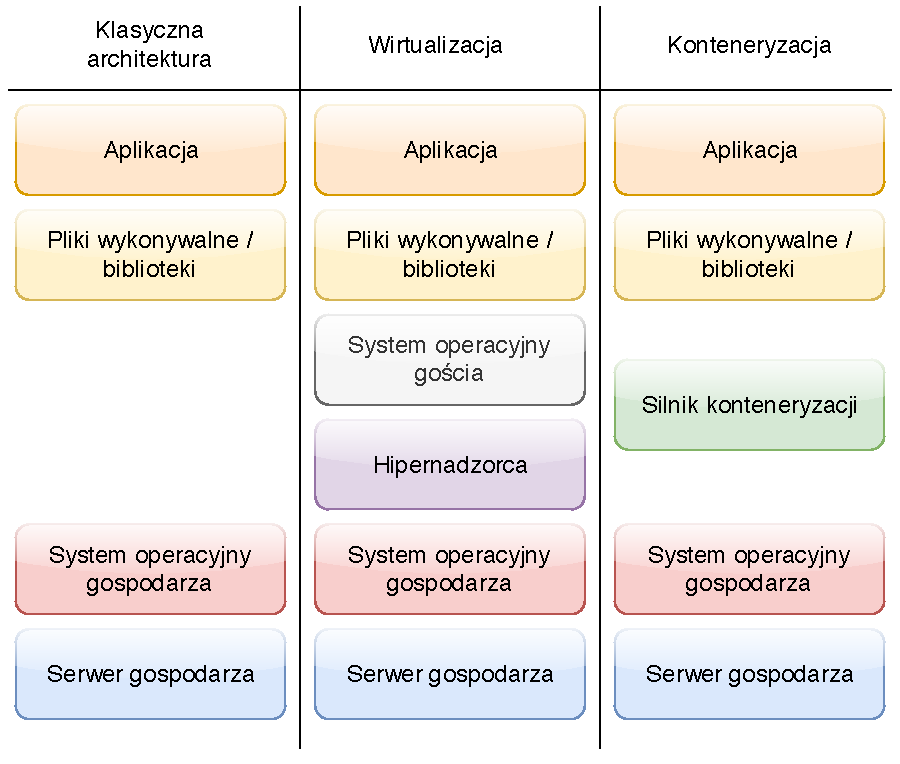
\includegraphics[width=\textwidth]{res/virtualizationAndContenerizatrionComparison}
\end{figure}
%%%%%%%%%%%%%%%%%%%%%%%%%%%%%%%%%%%%%%%%%%%%%%%%%%%%%%%%%%%%%%%%%%%%%%%%%%%%%%%%%%%%%
%%%%%%%%%%%%%%%%%%%%%%%%%%%%%%%%%%%%%%%%%%%%%%%%%%%%%%%%%%%%%%%%%%%%%%%%%%%%%%%%%%%%%
%%%%%%%%%%%%%%%%%%%%%%%%%%%%%%%%%%%%%%%%%%%%%%%%%%%%%%%%%%%%%%%%%%%%%%%%%%%%%%%%%%%%%
%%%%%%%%%%%%%%%%%%%%%%%%%%% STAN POCZATKOWY PROJEKTU %%%%%%%%%%%%%%%%%%%%%%%%%%%%%%%%
%%%%%%%%%%%%%%%%%%%%%%%%%%%%%%%%%%%%%%%%%%%%%%%%%%%%%%%%%%%%%%%%%%%%%%%%%%%%%%%%%%%%%
%%%%%%%%%%%%%%%%%%%%%%%%%%%%%%%%%%%%%%%%%%%%%%%%%%%%%%%%%%%%%%%%%%%%%%%%%%%%%%%%%%%%%
%%%%%%%%%%%%%%%%%%%%%%%%%%%%%%%%%%%%%%%%%%%%%%%%%%%%%%%%%%%%%%%%%%%%%%%%%%%%%%%%%%%%%

\chapter{Stan początkowy projektu}
\label{cha:pocz}

\section{Architektura}

\section{Budowanie} 
Niniejsza część pracy zawiera opis pierwotnego sposobu budowania aplikacji, wraz z zastosowanymi rozwiązaniami technologicznymi (struktura i zawartość plików CMake) oraz listą potencjalnych ograniczeń wynikających z dotychczasowego podejścia do budowania.

\paragraph*{Struktura plików CMake}\mbox{}\\
% Opisac co gdzie jest, za co odpowiadają poszczegolne szablony
Projekt w swojej oryginalnej postaci budowany był za pomocą narzędzia CMake w wersji \textbf{2.8}. Wyróżnić można było jeden nadrzędny plik \textit{CMakeLists.txt} znajdujący się w katalogu głownym projektu oraz pomniejsze pliki dla każdego z modułów. Rysunek przedstawia w uproszczeniu pierwotną strukturę projektu, z wyszczególnieniem plików odpowiedzialnych za jego budowanie.

\textbf{TODO: tutaj dac jakis fajny rysuneczek}












\paragraph*{Obsługa bibliotek zewnętrznych}\mbox{}\\
% Opisac, jak obsługiwany jest Boost, GSL, Caen



\paragraph*{Ograniczenia pierwotnego systemu budowania}\mbox{}\\
% Cos jeszcze dopisac, zrobic zeby sie to lepiej czytalo
Pierwotna wersja projektu narzuca daleko idące ograniczenia na sposób jego budowania. Najważniejszym z nich jest brak bezpośredniej możliwości zbudowania pojedynczych komponentów projektu. Listing \ref{lst:orig} przedstawia fragment oryginalnego pliku \textit{CMakeLists.txt} znajdującego się w katalogu głównym projektu. \textbf{TUTAJ REF DO PRACY PLUTECKIEGO} Plik ten pozwala na zbudowanie trzech aplikacji wchodzących w skład oprogramowania projektu GGSS: \textit{ggssrunner}, \textit{dimCS} oraz opcjonalnie \textit{ggsspector}. Jest to jedyny plik w całym projekcie zawierający wszystkie informacje konieczne do zbudowania wymienionych aplikacji - tzn. posiadający listę bibliotek, od których aplikacje te są zależne. Oznacza to, że niemożliwe jest zbudowanie aplikacji \textit{ggssrunner} jedynie za pomocą dedykowanego jej pliku \textit{CMakeLists.txt}. Zatem pomimo, iż struktura projektu jest zmodularyzowana jeśli chodzi o architekturę (oprogramowanie zostało podzielone na biblioteki), to niemożliwe jest (w prosty sposób, za pomocą dostarczonych plików \textit{CMakeLists.txt}) zbudowanie pojedynczych modułów projektu.

\begin{lstlisting}[language=bash, caption={Fragment oryginalnego pliku CMakeLists.txt znajdującego się w katalogu głównym pierwotnej wersji projektu}, label={lst:orig}]
# array with used libraries
set(PROJECTS
        logLib
        xmlLib
        utilsLib
        handleLib
        ThreadLib
        fifoLib
        FitLib
        OrtecMcbLib
        CaenHVLib
        ggssLib
        usbrmLib
        CaenN1470Lib
        mcaLib
        daemonLib
        )

foreach (singleproject ${PROJECTS})
        parse_directory(${singleproject})
endforeach(singleproject)

# executables
add_subdirectory (_ggss) # ggssrunner binary
add_subdirectory (_dimCS) #dimCS binary
if(BUILD_GGSSPECTOR)
    add_subdirectory (_ggsspector) #ggsspector binary
endif()
\end{lstlisting}

Budowanie projektu za pomocą pliku, którego fragment przedstawia listing \ref{lst:orig} opiera się na liście zależności przechowywanej w zmiennej \textit{PROJECTS}. Umożliwia to stosunkowo łatwe rozszerzanie projektu o nowe biblioteki - wystarczy dopisać nazwę katalogu z biblioteką do listy zależności. Wadą tego rozwiązania jest natomiast brak możliwości wywnioskowania zależności zachodzących w projekcie. Listing \ref{lst:origggss} przedstawia plik \textit{CMakeLists.txt} służący do budowania aplikacji \textit{ggssrunner}. Na podstawie tych dwóch plików można jedynie wywnioskować, że aplikacja \textit{ggssrunner} jest zależna od wszystkich bibliotek, których nazwy znaleźć można w zmiennej \textit{PROJECTS}. Nie ma natomiast możliwości identyfikacji zależności między samymi bibliotekami. Takie podejście utrudnia zrozumienie struktury projektu, co bezpośrednio prowadzi do problemów z jego rozwojem.

%% Dodac bardziej szczegolowy opis tego projektu
\begin{lstlisting}[language=bash, caption={Oryginalny plik CMakeLists.txt służacy budowania aplikacji ggssrunner.}, label={lst:origggss}]
project (_ggss)
add_executable (ggssrunner main)
target_link_libraries (ggssrunner ${PROJECTS})
install(TARGETS ggssrunner RUNTIME DESTINATION bin)
\end{lstlisting}




\section{Dostarczanie i uruchamianie}

\section{Kontrola wersji}


%%%%%%%%%%%%%%%%%%%%%%%%%%%%%%%%%%%%%%%%%%%%%%%%%%%%%%%%%%%%%%%%%%%%%%%%%%%%%%%%%%%%%
%%%%%%%%%%%%%%%%%%%%%%%%%%%%%%%%%%%%%%%%%%%%%%%%%%%%%%%%%%%%%%%%%%%%%%%%%%%%%%%%%%%%%
%%%%%%%%%%%%%%%%%%%%%%%%%%%%%%%%%%%%%%%%%%%%%%%%%%%%%%%%%%%%%%%%%%%%%%%%%%%%%%%%%%%%%
%%%%%%%%%%%%%%%%%%%%%%%%%%% STAN DOCELOWY PROJEKTU %%%%%%%%%%%%%%%%%%%%%%%%%%%%%%%%%%
%%%%%%%%%%%%%%%%%%%%%%%%%%%%%%%%%%%%%%%%%%%%%%%%%%%%%%%%%%%%%%%%%%%%%%%%%%%%%%%%%%%%%
%%%%%%%%%%%%%%%%%%%%%%%%%%%%%%%%%%%%%%%%%%%%%%%%%%%%%%%%%%%%%%%%%%%%%%%%%%%%%%%%%%%%%
%%%%%%%%%%%%%%%%%%%%%%%%%%%%%%%%%%%%%%%%%%%%%%%%%%%%%%%%%%%%%%%%%%%%%%%%%%%%%%%%%%%%%

\chapter{Stan docelowy projektu}
\label{cha:docel}

%%%%%%%%%%%%%%%%%%%%%%%%%%%%%%%%%%%%%%%%%%%%%%%%%%%%%%%%%%%%%%%%%%%%%%%%%%%%%%%%%%%%%
%%%%%%%%%%%%%%%%%%%%%%%%%%%%%%%%%%%%%%%%%%%%%%%%%%%%%%%%%%%%%%%%%%%%%%%%%%%%%%%%%%%%%
%%%%%%%%%%%%%%%%%%%%%%%%%%%%%%%%%%%%%%%%%%%%%%%%%%%%%%%%%%%%%%%%%%%%%%%%%%%%%%%%%%%%%
%%%%%%%%%%%%%%%%%%%%%%%%%%% OGRANICZENIA INFRASTRUKTURY %%%%%%%%%%%%%%%%%%%%%%%%%%%%%
%%%%%%%%%%%%%%%%%%%%%%%%%%%%%%%%%%%%%%%%%%%%%%%%%%%%%%%%%%%%%%%%%%%%%%%%%%%%%%%%%%%%%
%%%%%%%%%%%%%%%%%%%%%%%%%%%%%%%%%%%%%%%%%%%%%%%%%%%%%%%%%%%%%%%%%%%%%%%%%%%%%%%%%%%%%
%%%%%%%%%%%%%%%%%%%%%%%%%%%%%%%%%%%%%%%%%%%%%%%%%%%%%%%%%%%%%%%%%%%%%%%%%%%%%%%%%%%%%

\chapter{Ograniczenia dostępnej infrastruktury}
\label{cha:ogra}
Z uwagi na silny związek oprogramowania GGSS z infrastrukturą CERN oraz wymóg zapewnienia możliwości budowania projektu na należących do niej maszynach, przed autorami postawiony został szereg ograniczeń związanych z możliwymi do użycia technologiami oraz sposobem wykonywania pewnych operacji. Niniejszy rozdział stanowi opis najważniejszych z tych ograniczeń z uwzględnieniem ich wpływu na obraną przez autorów pracy ścieżkę rozwoju projektu.


\section{Ograniczone uprawnienia w środowisku docelowym}


\section{Wersje kompilatorów i interpreterów}
Dostępne wersje kompilatorów i interpreterów stanowią jeden z kluczowych czynników, który należy uwzględnić podczas wprowadzania zmian w istniejącym systemie, ponieważ definiują one możliwy do wykorzystania podzbiór technologii. W kontekście systemu GGSS ograniczenia te dotyczą przede wszystkim kompilatora języka C++ oraz interpretera języka Python. 

\paragraph*{Wersja kompilatora języka C++}\mbox{}\\
Dostępna w ramach infrastruktury projektu wersja kompilatora języka C++ to \textbf{g++ (GCC) 4.8.5}. Wspiera ona w pełni standard C++11, czyli funkcjonalności takie, jak referencje do r-wartości, wyrażenia lambda czy zakresowa pętla for \cite{GCC48}. Wersja ta nie wspiera niestety nowszych wydań języka (C++14/17).

\paragraph*{Wersja interpretera języka Python}\mbox{}\\
Domyślną wersją Pythona jest \textbf{Python 2.7.5}, jednak dostępny jest również Python 3 (w wersji \textbf{Python 3.6.8}). Z uwagi na wspomniany wcześniej koniec oficjalnego wsparcia dla Pythona 2, który ma nadejść wraz z początkiem 2020 roku, naturalnym jest więc wybór wersji 3. Infrastruktura projektu posiada jednak znaczące braki jeśli chodzi o dostępne dla wersji 3 biblioteki zewnętrzne - domyślnie nie jest np. dostępna biblioteka \textit{Beautiful Soup}, slużąca do przetwarzania dokumentów w formacie HTML. Niektóre popularne bibliteki i frameworki (np. \textit{PyTest} - wykorzystywany do przeprowadzania testów oprogramowania) nie są dostępne dla obu wersji Pythona. Taka sytuacja wymusza więc wykorzystanie narzędzia \textit{virtualenv} w celu ich instalacji w odizolowanym środowisku, nie mającym wpływu na infrastrukturę CERN-u.

\section{Wersja narzędzia budującego CMake}
Dostępna wersja narzędzia CMake stanowiła zdaniem autorów największe ograniczenie w czasie prac nad projektem. Na maszynach docelowych dostępna jest jedynie stara wersja \textbf{2.8.12.2}. Nowsza wersja (\textbf{3.14.6}) dostępna jest na niektórych z komputerów, jednak z uwagi na konieczność zachowania kompatybilności ze wspomnianymi maszynami docelowymi, nie było możliwe jej użycie. Stosowanie wersji o numerze niższym od \textbf{3.0} skutkuje szeregiem ograniczeń - brakuje w niej wielu funkcjonalności pozwalających na stosowanie ogólnoprzyjętych dziś praktyk, jak np. określenie zakresu wersji narzedzia CMake, w którym powinna mieścić się używana wersja, by projekt można było bez problemu zbudować, czy wsparcie dla instrukcji \textit{target\_link\_directories} \cite{NewInCMake}.

\section{Związek projektu z wersją jądra systemu}


%%%%%%%%%%%%%%%%%%%%%%%%%%%%%%%%%%%%%%%%%%%%%%%%%%%%%%%%%%%%%%%%%%%%%%%%%%%%%%%%%%%%%
%%%%%%%%%%%%%%%%%%%%%%%%%%%%%%%%%%%%%%%%%%%%%%%%%%%%%%%%%%%%%%%%%%%%%%%%%%%%%%%%%%%%%
%%%%%%%%%%%%%%%%%%%%%%%%%%%%%%%%%%%%%%%%%%%%%%%%%%%%%%%%%%%%%%%%%%%%%%%%%%%%%%%%%%%%%
%%%%%%%%%%%%%%%%%%%%%%%%%%% WYKONANE PRACE %%%%%%%%%%%%%%%%%%%%%%%%%%%%%%%%%%%%%%%%%%
%%%%%%%%%%%%%%%%%%%%%%%%%%%%%%%%%%%%%%%%%%%%%%%%%%%%%%%%%%%%%%%%%%%%%%%%%%%%%%%%%%%%%
%%%%%%%%%%%%%%%%%%%%%%%%%%%%%%%%%%%%%%%%%%%%%%%%%%%%%%%%%%%%%%%%%%%%%%%%%%%%%%%%%%%%%
%%%%%%%%%%%%%%%%%%%%%%%%%%%%%%%%%%%%%%%%%%%%%%%%%%%%%%%%%%%%%%%%%%%%%%%%%%%%%%%%%%%%%

\chapter{Wykonane prace}
\label{cha:prace}

\section{Wykorzystanie funkcjonalności portalu Gitlab wspierających zarządzanie projektem}

\section{Migracja projektu do systemu kontroli wersji Git i zmiany w architekturze}

\section{Zastosowanie podejścia CI/CD}
% Czym jest CI/CD
% Realiacja za pomocą platformy gitLab
%   - mozliwe opcje, czemu nie autodevops
%   - pipeline (z przykladem)
%   - artefakty i ich znaczenie w GGSS
%   - pliki .yml (z przykladem)

\section{Zmiana sposobu budowania aplikacji}
% Zarys rozwiazania
% Szablony + Boost + GSL
% Budowanie bibliotek
% Budowanie aplikacji
% DIM - skrypt do pobierania, budowanie jak external_project
% Skrypty do budowania calosci (+ sposoby budowania) + glowny CMake

\section{Budowanie i dystrybucja sterownika oraz aplikacji testującej}

\section{Maszyna wirtualna oraz konteneryzacja - Docker}

\section{Pomniejsze prace}
\subsection{Integracja bibliotek napisanych w języku C z aplikacją w C++}
\subsection{Integracja zewnętrznej biblioteki dynamicznej z użyciem narzędzia CMake}

\section{Dokumentacja projektu}
% Czemu potrzebna
% Realizacja - pliki README.md, one-linery

%%%%%%%%%%%%%%%%%%%%%%%%%%%%%%%%%%%%%%%%%%%%%%%%%%%%%%%%%%%%%%%%%%%%%%%%%%%%%%%%%%%%%
%%%%%%%%%%%%%%%%%%%%%%%%%%%%%%%%%%%%%%%%%%%%%%%%%%%%%%%%%%%%%%%%%%%%%%%%%%%%%%%%%%%%%
%%%%%%%%%%%%%%%%%%%%%%%%%%%%%%%%%%%%%%%%%%%%%%%%%%%%%%%%%%%%%%%%%%%%%%%%%%%%%%%%%%%%%
%%%%%%%%%%%%%%%%%%%%%%%%%%% DALSZY ROZWOJ PROJEKTU %%%%%%%%%%%%%%%%%%%%%%%%%%%%%%%%%%
%%%%%%%%%%%%%%%%%%%%%%%%%%%%%%%%%%%%%%%%%%%%%%%%%%%%%%%%%%%%%%%%%%%%%%%%%%%%%%%%%%%%%
%%%%%%%%%%%%%%%%%%%%%%%%%%%%%%%%%%%%%%%%%%%%%%%%%%%%%%%%%%%%%%%%%%%%%%%%%%%%%%%%%%%%%
%%%%%%%%%%%%%%%%%%%%%%%%%%%%%%%%%%%%%%%%%%%%%%%%%%%%%%%%%%%%%%%%%%%%%%%%%%%%%%%%%%%%%

\chapter{Dalsza ścieżka rozwoju projektu}
\label{cha:dalsze}

\section{Wprowadzenie zautomatyzowanego systemu testowania projektu}
\section{Migracja do nowego standardu języka C++}
\section{Automatyzacja procesu publikowania produktu}


\chapter{Testy nowej wersji oprogramowania}
\label{cha:test}
Niniejszy rozdział zawiera opis testów systemu \gls*{ggss} przeprowadzonych na koniec trwania prac związanych z~jego oprogramowaniem. Celem testów była weryfikacja poprawności działania czterech konfiguracji programu \textit{ggssrunner}: wersja deweloperska (\textit{debug}) ze statycznie linkowaną biblioteką \textit{Boost}, wersja deweloperska z~dynamicznie linkowaną biblioteką \textit{Boost} oraz analogiczne wersje produkcyjne (\textit{release}). Z~uwagi na powtarzalny charakter procesu testowania zaprezentowany zostanie jedynie przebieg testów dla wersji \textbf{deweloperskiej ze statycznie linkowaną biblioteką Boost}. 

\section{Przebieg testu}
Ze względu na fakt, że środowisko w~którym osadzony jest program \textit{ggssrunner} jest ciągle monitorowane, pierwszym krokiem było umieszczenie informacji o~przeprowadzaniu testów w~dedykowanym do tego celu systemie \textbf{ELisA (Electronic Logbook for Information Storage for Atlas)}.

\begin{figure}[H]
\centering
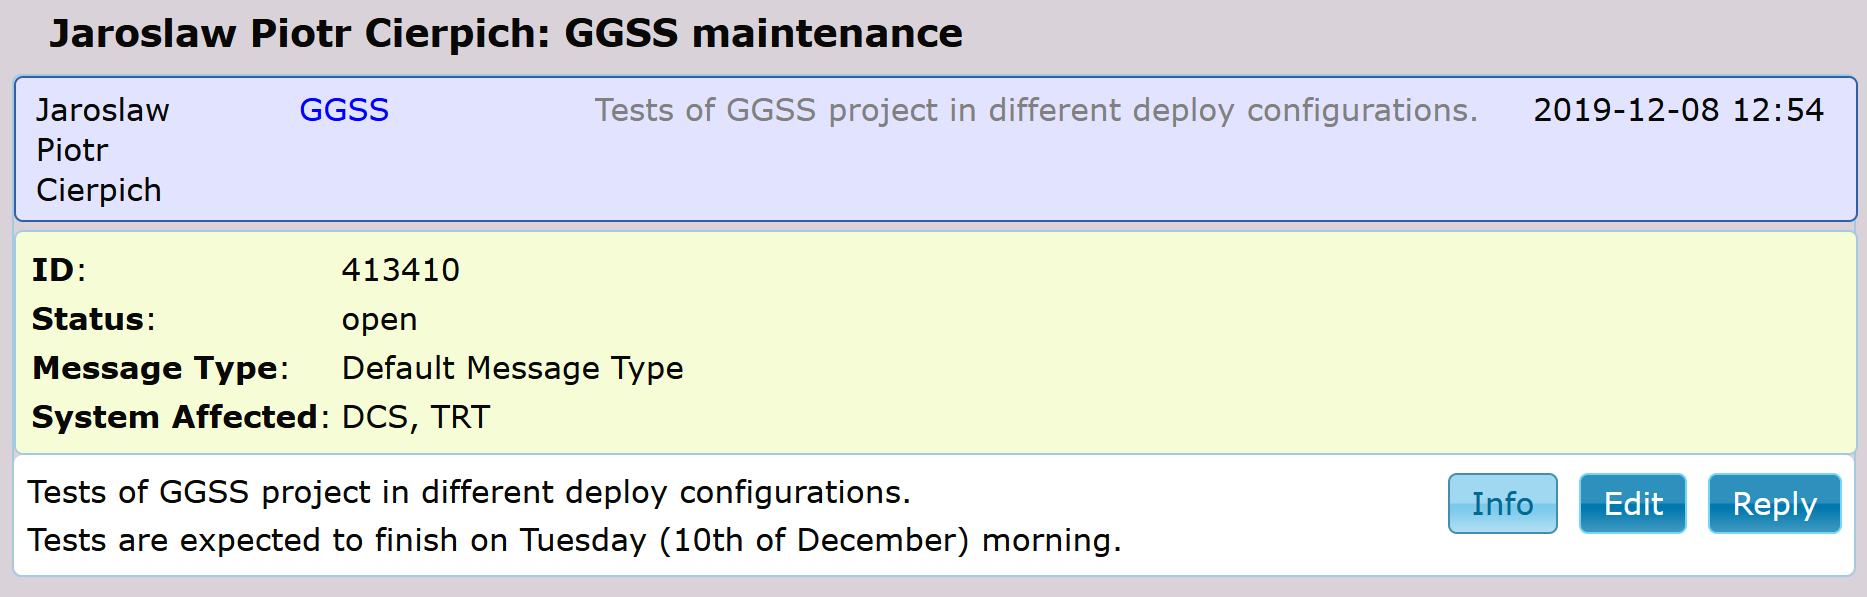
\includegraphics[width=\textwidth]{res/png/elisa}
\caption{Informacja o~przeprowadzaniu testów w~systemie ELisA}
\label{fig:elisa}
\end{figure}

Pliki wykonywalne aplikacji \textit{ggssrunner} wygenerowane zostały za pomocą przygotowanego przez autorów środowiska CI/CD. Zostały one umieszczone na komputerze produkcyjnym. Kolejnym krokiem było zalogowanie się do panelu \textit{WinCC OA} służącego do monitorowania działania detektora ATLAS oraz wybranie panelu odpowiedzialnego za dostarczanie informacji o~systemie \gls*{ggss}. 

\begin{figure}[H]
\centering
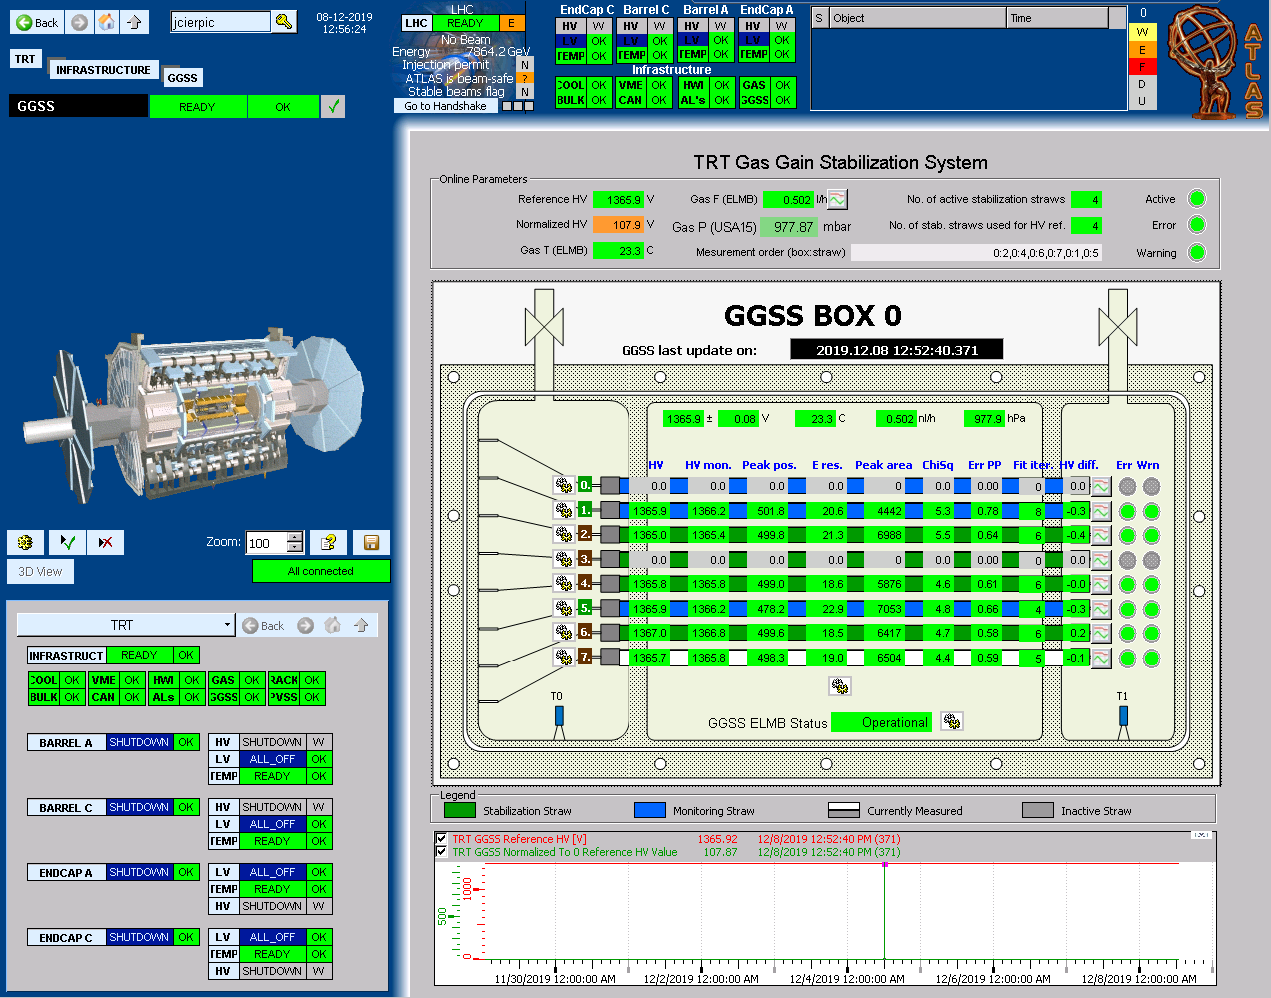
\includegraphics[width=\textwidth]{res/png/ggssStraw}
\caption{Panel WinCC OA monitorujący działanie systemu \gls*{ggss}}
\label{fig:ggss}
\end{figure}

\newpage
Następnym etapem było przeprowadzenie procesu wyłączania systemu \gls*{ggss} za pomocą przycisku \textit{Stop} znajdującego się na dedykowanym panelu konfiguracyjnym ukazanym na Rys. \ref{fig:ggsspanel}. 

\begin{figure}[H]
\centering
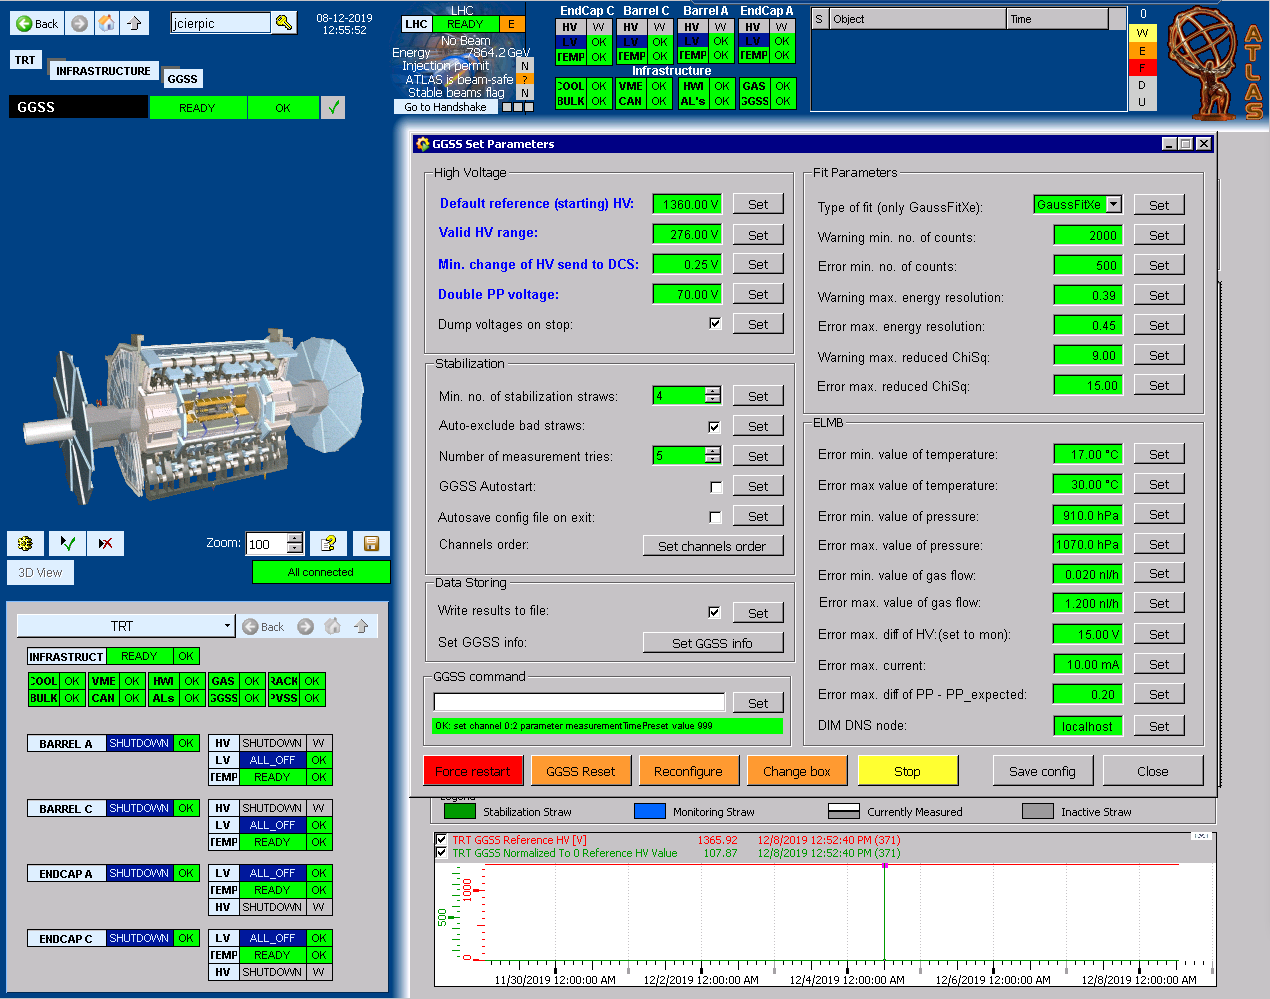
\includegraphics[width=\textwidth]{res/png/ggssConfig}
\caption{Panel konfiguracyjny systemu \gls*{ggss} podczas działania systemu}
\label{fig:ggsspanel}
\end{figure}


\newpage
Po wyłączeniu systemu należało również przerwać działanie poprzedniej wersji aplikacji \textit{ggssrunner} za pomocą skryptu \textit{ggss\_monitor.sh} (listing \ref{lst:ggssstop}). Za pomocą tego skryptu został również potwierdzony stan aplikacji po wyłączeniu.


\begin{lstlisting}[language=Cmd, caption={Zatrzymanie działania aplikacji \textit{ggssrunner}}, label={lst:ggssstop}]
user@host:~$ ./ggss_monitor.sh check
ggssrunner is running.

user@host:~$ ./ggss_monitor.sh stop
ggssrunner: no process found
Creating lock /localdisk/ggss/bin/autostartggss.lock

user@host:~$ ./ggss_monitor.sh check
ggssrunner is NOT running. /localdisk/ggss/bin/autostartggss.lock exists. Remove it or start GGSS manually
\end{lstlisting}



Po wykonaniu wyżej wymienionych czynności podmieniony został plik wykonywalny aplikacji \textit{ggssrunner} na przygotowany przez autorów. Zmiana została wykonana poprzez modyfikacje \textbf{dowiązania symbolicznego}. Następnie aplikacja uruchomiona została ponownie za pomocą skryptu \textit{ggss\_monitor.sh} (listing \ref{lst:ggssstart}) oraz z~poziomu panelu \textit{WinCC OA}. Stan panelu monitorującego system \gls*{ggss} jest widoczny na Rys. \ref{fig:ggssafterstart}.

\begin{lstlisting}[language=Cmd, caption={Ponowne uruchomienie aplikacji \textit{ggssrunner}}, label={lst:ggssstart}]
user@host:~$ ./ggss_monitor.sh remove_lock
Removing lock /localdisk/ggss/bin/autostartggss.lock

user@host:~$ ./ggss_monitor.sh check
ggssrunner is NOT running.

user@host:~$ ./ggss_monitor.sh check_start
\end{lstlisting}

\begin{figure}
\centering
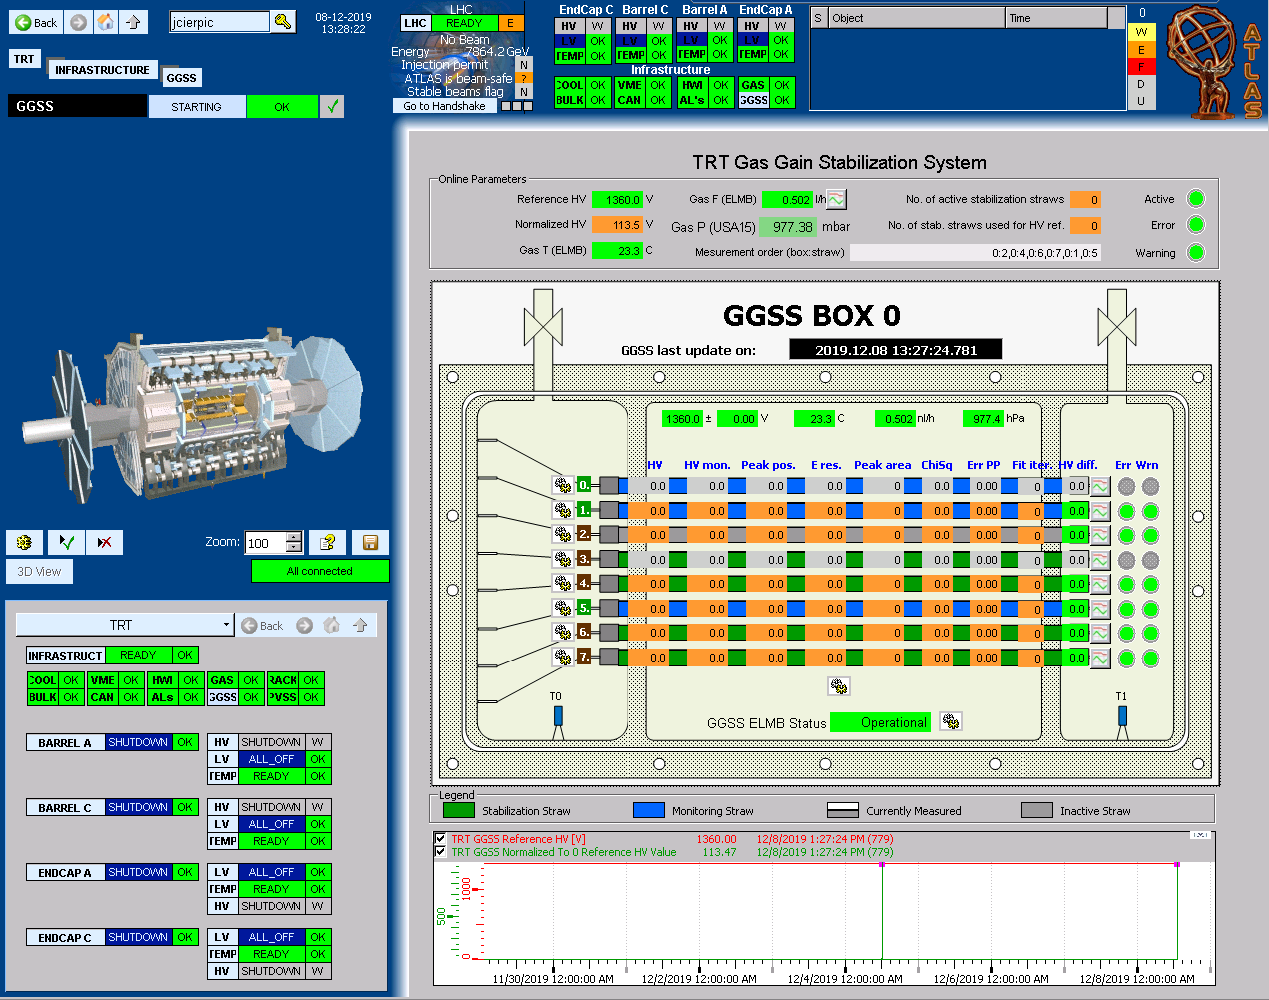
\includegraphics[width=\textwidth]{res/png/ggssPoStarcie}
\caption{Panel WinCC OA monitorujący działanie systemu \gls*{ggss} po ponownym uruchomieniu systemu (widoczny w~lewym górnym rogu stan \textit{STARTING})}
\label{fig:ggssafterstart}
\end{figure}

\newpage
Dodatkowo użyty został skrypt pozwalający na monitorowanie zużycia zasobów pamięci przez aplikację (listing \ref{lst:ggssmem1}). Sposób użycia oraz fragment generowanego przez ten skrypt wyjścia przedstawia listing \ref{lst:ggssmem2}. 

\begin{lstlisting}[language=bash, caption={Skrypt \textit{check\_mem\_ggssrunner.sh} służacy do monitorowania pamięci używanej przez aplikację \textit{ggssrunner}}, label={lst:ggssmem1}]
#!/bin/bash
while true
do
    ps afux | egrep " ./ggssrunner" | awk -v date="$(date +"%Y.%m.%d %H:%M:%S")" '{print date, $5}'
    sleep 1m
done
\end{lstlisting}


\begin{lstlisting}[language=Cmd, caption={Wywołanie oraz fragment wyjścia skryptu \textit{check\_mem\_ggssrunner.sh} służacego do monitorowania pamięci używanej przez aplikację \textit{ggssrunner}}, label={lst:ggssmem2}]
user@host:~$ ./check_mem_ggssrunner.sh
2019.12.08 15:15:26 638800
2019.12.08 15:16:26 638800
2019.12.08 15:17:26 638800
2019.12.08 15:18:26 638800
2019.12.08 15:19:26 638800
2019.12.08 15:20:27 638800
2019.12.08 15:21:27 638800
2019.12.08 15:22:27 638800
\end{lstlisting}

W takim stanie system pozostawiony został na dłuższy (ponad 6 godzin) czas. Idea testu polegała na sprawdzeniu, czy przez ten czas działanie systemu pozostanie stabilne i~nie pojawią się żadne błędy.

\section{Wyniki testu}
Test każdej z~przygotowanych konfiguracji trwał \textbf{ponad 6 godzin}. Tabela \ref{tab:wyniki} przedstawia rezultaty.

\begin{table}[]
\begin{tabular}{|c|c|c|c|}
\hline
\rowcolor[HTML]{ECF4FF} 
\textbf{\begin{tabular}[c]{@{}c@{}}Konfiguracja \\ (debug/release)\end{tabular}} & \textbf{\begin{tabular}[c]{@{}c@{}}Sposób linkowania \\ biblioteki Boost\end{tabular}} & \textbf{Wygenerowane błędy}                                                              & \textbf{\begin{tabular}[c]{@{}c@{}}Zaalokowana \\ pamięć\end{tabular}} \\ \hline
debug                                                                            & statyczne                                                                              & brak                                                                                     & stała                                                                  \\ \hline
release (-O3)                                                                    & statyczne                                                                              & \begin{tabular}[c]{@{}c@{}}błąd zarejestrowany\\ dla całego systemu \\ GGSS\end{tabular} & stała                                                                  \\ \hline
release (-O2)                                                                    & statyczne                                                                              & brak                                                                                     & stała                                                                  \\ \hline
debug                                                                            & dynamiczne                                                                             & brak                                                                                     & stała                                                                  \\ \hline
release (-O3)                                                                    & dynamiczne                                                                             & \begin{tabular}[c]{@{}c@{}}błąd zarejestrowany\\ dla konkretnej\\ słomki\end{tabular}    & stała                                                                  \\ \hline
\end{tabular}
\caption{Wyniki testów systemu \gls*{ggss} po wprowadzonych zmianach}
\label{tab:wyniki}
\end{table}

Podczas przeprowadzania testów wersji produkcyjnej zostały wykryte błędy w~działaniu, co zostało zakomunikowane na panelu WinCC OA. Błędy te pojawiły się zarówno na poziomie całego systemu (Rys. \ref{fig:ggssErrorScada}), jak i~pojedynczej słomki (Rys. \ref{fig:ggssErrorStrawScada}). Pojawienie się błędów było skutkiem zastosowania w~czasie kompilacji flagi optymalizacji \textit{-O3}. Jest to domyślna flaga stosowana przez narzędzie \gls*{cmake} dla wersji produkcyjnej. Podczas kompilacji aplikacji \textit{ggssrunner} w~takiej konfiguracji widoczne były dwa ostrzeżenia, zatem błędy nie były dla autorów zaskoczeniem. Flaga \textit{-O3} oznacza agresywną politykę optymalizacji, co często prowadzi do zmiany zachowania aplikacji. Została więc wprowadzona zmiana w~sposobie kompilacji aplikacji w~wersji produkcyjnej - flaga ta została zastąpiona przez jej łagodniejszy i~stabilniejszy odpowiednik \textit{-O2}, powszechnie wykorzystywany do tworzenia wersji produkcyjnych oprogramowania. Testy wykonane z~użyciem tej flagi nie wyprodukowały żadnych błędów. 

Testy wersji deweloperskiej (w obu konfiguracjach) odbyły się bez problemów - nie zostały wygenerowane żadne błędy ani ostrzeżenia. 

W każdym z~przypadków ilość zaalokowanej przez program pamięci pozostawała stała przez cały czas trwania testu. Oznacza to brak znaczących problemów z~zarządzaniem pamięcią (takich jak wycieki pamięci).

Wyniki przeprowadzonych testów stanowią potwierdzenie poprawności wprowadzonych przez autorów zmian w~systemie. 

\begin{figure}
\centering
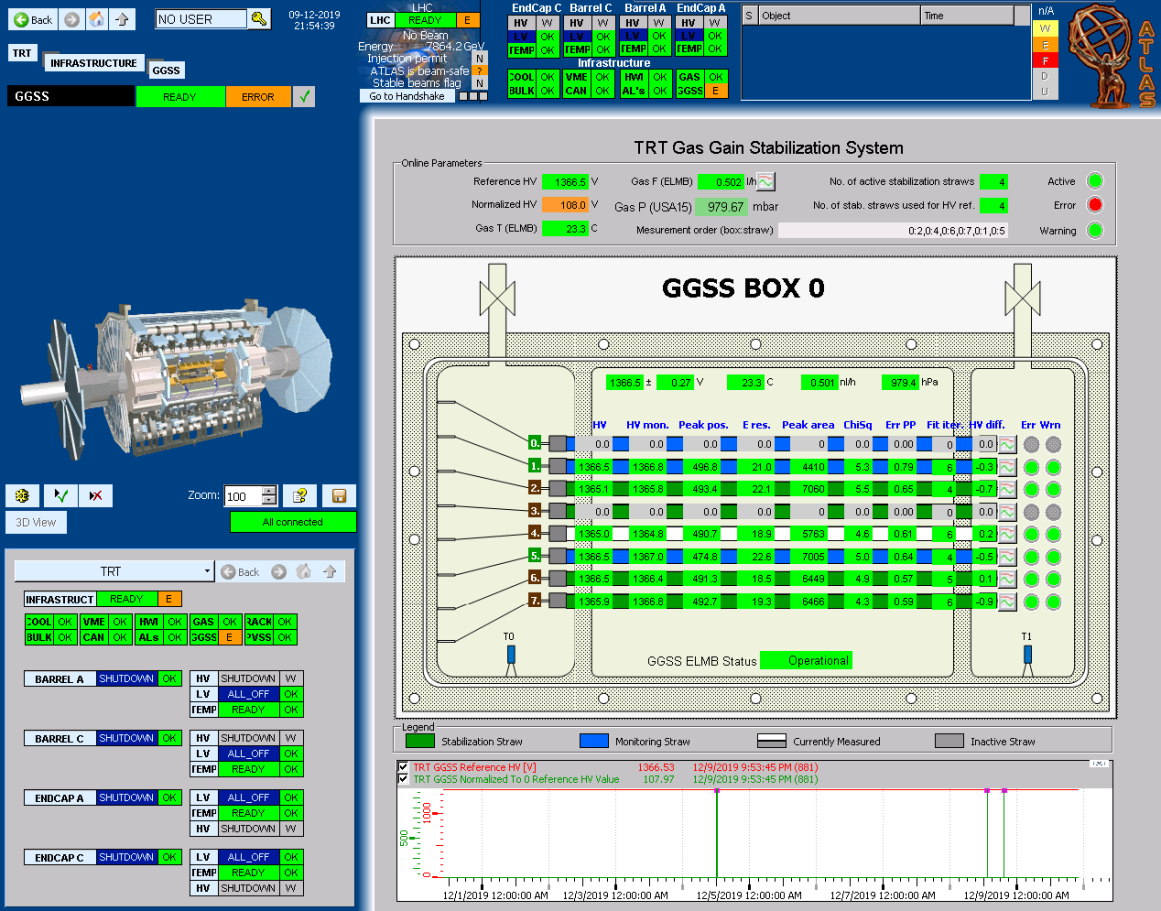
\includegraphics[width=\textwidth]{res/png/ggssError}
\caption{Błąd w~działaniu aplikacji \textit{ggssrunner} na poziomie całego systemu widoczny w~panelu WinCC OA (czerwone koło w~prawym górnym rogu panelu \gls*{ggss})}
\label{fig:ggssErrorScada}
\end{figure}


\begin{figure}
\centering
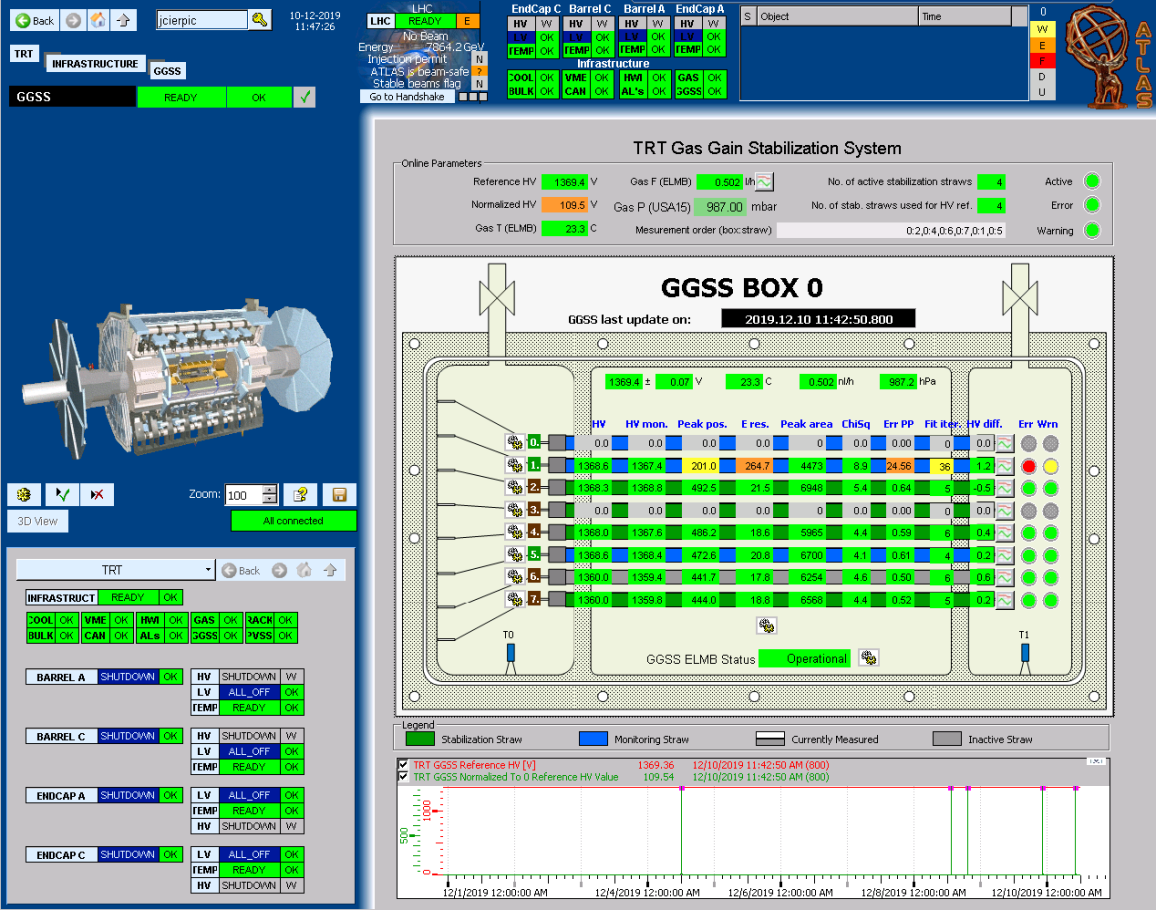
\includegraphics[width=\textwidth]{res/png/errStraw}
\caption{Błąd w~działaniu aplikacji \textit{ggssrunner} na poziomie pojedynczej słomki widoczny w~panelu WinCC OA (czerwone koło obok drugiej słomki)}
\label{fig:ggssErrorStrawScada}
\end{figure}

\chapter{Podsumowanie oraz wnioski}
\label{cha:summary}


\appendix
\chapter{Dodatki/Appendixes}
\label{cha:app}

\section{Adding new modules to the project using existing CMake templates}
\section{Preparing virtual machine to work as a runner}


\printbibliography

\end{document}